% !Mode:: "TeX:UTF-8"
% Translator: Shenjian Zhao
\chapter{\glsentrytext{DL}的正则化}
\label{chap:regularization_for_deep_learning}
\gls{ML}中的一个核心问题是设计不只在训练数据表现好,而且能在新输入上泛化的算法。
在\gls{ML}中,许多策略被明确设计为以增大训练误差为代价来减少测试误差。
这些策略统称为\gls{regularization}。
正如我们会看到的,\gls{DL}工作者可以使用许多形式的\gls{regularization}。
事实上,开发更有效的\gls{regularization}策略已成为本领域的主要研究工作之一。

\chapref{chap:machine_learning_basics}介绍了\gls{generalization}、\gls{underfitting}、\gls{overfitting}、\gls{bias_sta}、\gls{variance}和\gls{regularization}的基本概念。
如果你不熟悉这些概念,请参考该章节再继续阅读本章。

在本章中,我们会更详细地描述\gls{regularization},重点描述深度模型(或模块)的\gls{regularization}策略。

本章某些节涉及\gls{ML}中的标准概念。
如果你已经熟悉了这些概念,可以随意跳过相关章节。
然而,本章的大多数内容涉及这些基本概念到特定\gls{NN}的扩展。

在\secref{sec:regularization},我们将\gls{regularization}定义为``旨在减少学习算法的\gls{generalization}误差而不是训练误差的修改''。
目前有许多\gls{regularization}策略。
有些向\gls{ML}模型添加额外的约束,如增加对参数的限制。
有些向\gls{objective_function}增加额外项,对应于参数值的软约束。
如果仔细选择,这些额外的约束和惩罚可以改善模型在测试集上的表现。
有时,这些约束和惩罚设计为编码特定类型的先验知识。
其他时候,这些约束和惩罚的目的是表达对简单模型的一般偏好,以便提高\gls{generalization}能力。
有时候,惩罚和约束对于确定欠定的问题是必要的。
其他形式的\gls{regularization},如\gls{ensemble}方法,结合多个假说来解释训练数据。

% -- 221 --

在\gls{DL}的背景下,大多数\gls{regularization}策略都基于对\gls{estimator}进行\gls{regularization}。
\gls{estimator}的\gls{regularization}以\gls{bias_sta}的增加换取\gls{variance}的减少。
一个有效的\gls{regularization}是有利的``交易'',也就是能显著减少\gls{variance}而不过度增加\gls{bias_sta}。
我们在\chapref{chap:machine_learning_basics}中讨论\gls{generalization}和\gls{overfitting}时,主要侧重模型族训练的3个情形:(1)不包括真实的数据生成过程——对应于\gls{underfitting}和\gls{bias_sta}引入,(2)匹配真实数据生成过程,(3)除了包含真实的数据生成过程,还包含了许多其他可能的生成过程——\gls{variance}(而不是\gls{bias_sta})主导的\gls{overfitting}。
\gls{regularization}的目标是使模型从第三种情况进入到第二个情况。

在实践中,过于复杂的模型族不一定包括目标函数或真实数据生成过程,甚至近似的都不包含。
我们几乎从来无法知晓真实数据的生成过程,所以我们永远不知道被估计的模型族是否包括生成过程。
然而,\gls{DL}算法的大多数应用都是针对这样的领域,其中真实数据的生成过程几乎可以肯定是模型族之外。
\gls{DL}算法通常应用于极为复杂的领域,如图像、音频序列和文本,本质上这些领域的真正生成过程涉及模拟整个宇宙。
从某种程度上说,我们总是持方枘(数据生成过程)而欲内圆凿(我们的模型族)。

这意味着控制模型的复杂性不是找到合适规模的模型(带有正确的参数个数)这样一个简单的事情。
相反,我们可能会发现,在实际的深度学习场景中我们几乎总是发现
,最好的拟合模型(最小化\gls{generalization}误差的意义上)是一个适当\gls{regularization}的大型模型。

现在我们回顾几种创建这样的大型深度\gls{regularization}模型的策略。

% -- 222 --

\section{参数范数惩罚}
\label{sec:parameter_norm_penalties}
\gls{regularization}在\gls{DL}的出现前就已经应用了数十年。
\gls{linear_model},如\gls{linear_regression}和\gls{logistic_regression}可以使用简单、直接有效的\gls{regularization}策略。

许多\gls{regularization}方法通过对\gls{objective_function}$J$添加一个参数范数惩罚$\Omega(\Vtheta)$,以限制模型(如\gls{NN}、\gls{linear_regression}或\gls{logistic_regression})的学习能力。
我们将正则化后的\gls{objective_function}记为$\tilde{J}$:
\begin{align}
 \tilde{J}(\Vtheta;\MX, \Vy) = J(\Vtheta;\MX, \Vy) + \alpha \Omega(\Vtheta),
\end{align}
其中$\alpha \in [0, \infty)$是权衡范数惩罚项$\Omega$和标准\gls{objective_function}$J(\MX;\Vtheta)$相对贡献的超参数。
将$\alpha$设为0就是没有\gls{regularization}。
越大的$\alpha$,对应于越多的\gls{regularization}惩罚。

当我们的训练算法最小化\gls{regularization}后的\gls{objective_function}$\tilde{J}$时,它会降低原始目标$J$关于训练数据的误差并同时减小参数$\Vtheta$的规模(或在某些衡量下参数子集的规模)。
参数规范$\Omega$的不同选择可以导致不同优先解。
在本节中,我们讨论各种范数惩罚模型参数时的影响。

在探究不同范数的\gls{regularization}表现之前,我们需要提一下,在神经网络中我们通常只对每一层仿射变换的\emph{权重}做惩罚而不对\gls{bias_aff}做正则惩罚。
通常使用比拟合权重更少的数据,就能精确拟合\gls{bias_aff}。
每个权重指定两个变量如何相互作用。
需要在各种条件下观察这两个变量才能拟合权重。
而每个\gls{bias_aff}仅控制一个单变量。
这意味着,我们不对其进行\gls{regularization}也不会引起太大\gls{variance}。
另外,\gls{regularization}的\gls{bias_aff}参数可能会引起显著的\gls{underfitting}。
因此,我们使用向量$\Vw$表示所有应受范数惩罚影响的权重,而向量$\Vtheta$表示所有参数(包括$\Vw$和不用\gls{regularization}的参数)。

在\gls{NN}的情况下,有时希望对网络的每个层使用单独的惩罚,并分配不同的$\alpha$系数。
搜索多个正确超参数的代价很大,因此在所有层使用相同\gls{weight_decay}以减少搜索空间是合理的。

% -- 223 --

\subsection{$L^2$参数\glsentrytext{regularization}}
\label{sec:l2_parameter_regularization}
在\secref{sec:capacity_overfitting_and_underfitting}中我们已经看到最简单和最常见的参数范数惩罚是,通常被称为\firstgls{weight_decay}的$L^2$参数范数惩罚。
这个\gls{regularization}策略通过向\gls{objective_function}添加一个正则项$\Omega(\Vtheta) = \frac{1}{2} \norm{\Vw}_2^2$,使权重更加接近原点\footnote{更一般地,我们可以将参数\gls{regularization}为接近空间中的任意特定点,令人惊讶的是仍有\gls{regularization}效果,并且更接近真实值将获得更好的结果。
当我们不知道正确的值应该是正还是负,零是有意义的默认值。
由于将模型参数\gls{regularization}为零的情况更常见,我们将关注这种特殊情况。}。
在其他学术圈,$L^2$也被称为\gls{ridge_regression}或\gls{tikhonov_regularization}。

我们可以通过研究\gls{regularization}化后\gls{objective_function}的\gls{gradient}洞察一些\gls{weight_decay}的\gls{regularization}表现。
为了简单起见,我们假定其中没有\gls{bias_aff}参数,因此$\Vtheta$就是$\Vw$。
这样一个模型具有以下总的\gls{objective_function}:
\begin{align}
  \tilde{J}(\Vw;\MX, \Vy) =\frac{\alpha}{2} \Vw^\top \Vw +  J(\Vw;\MX, \Vy),
\end{align}
与之对应的\gls{gradient}为
\begin{align}
 \nabla_{\Vw} \tilde{J}(\Vw;\MX,\Vy) =\alpha \Vw +  \nabla_{\Vw} J(\Vw;\MX, \Vy).
\end{align}
使用单步\gls{gradient}下降更新的权重,即执行以下更新:
\begin{align}
 \Vw \leftarrow \Vw - \epsilon(\alpha \Vw + \nabla_{\Vw} J(\Vw;\MX, \Vy)).
\end{align}
换种写法就是:
\begin{align}
 \Vw \leftarrow (1-\epsilon \alpha)\Vw - \epsilon \nabla_{\Vw} J(\Vw;\MX, \Vy).
\end{align}
我们可以看到,在加入\gls{weight_decay}后会修改学习规则——在每一步执行通常的\gls{gradient}更新之前对权重向量乘以一个常数因子以收缩权重向量。
这是单一步骤发生的变化。
但是,在训练的整个过程会发生什么?

% -- 224 --

我们进一步简化分析,令$\Vw^*$为没有\gls{regularization}的\gls{objective_function}取得最小训练误差的权重向量,即$\Vw^* = \argmin_{\Vw} J(\Vw)$, 并在$\Vw^*$的邻域作二次近似。
如果\gls{objective_function}确实是二次的(如以均方误差拟合\gls{linear_regression}模型的情况下),则该近似是完美的。
近似的$\hat J(\Vtheta)$如下
\begin{align}
 \hat J(\Vtheta) = J(\Vw^*) + \frac{1}{2}(\Vw - \Vw^*)^\top \MH (\Vw - \Vw^*),
\end{align}
其中$\MH$是$J$在$\Vw^*$处计算的\gls{hessian}矩阵(关于$\Vw$)。
因为$\Vw^*$被定义为最小,即梯度消失为0,所以该二次近似中没有一阶项。
同样,因为$\Vw^*$是$J$的一个最小点,我们可以得出$\MH$是半正定的结论。

当$\hat J$取最小时,其梯度
\begin{align}
\label{eq:gradient}
  \nabla_{\Vw} \hat{J}(\Vw) = \MH (\Vw - \Vw^*)
\end{align}
为0。

为了研究\gls{weight_decay}的影响,我们将\gls{weight_decay}的梯度加到\eqnref{eq:gradient}中。 
现在我们要找\gls{regularization}版本$\hat J$的最小值。
我们使用变量$\tilde{\Vw}$表示最小值的位置:
\begin{align}
 \alpha \tilde{\Vw} + \MH (\tilde{\Vw} - \Vw^*) = 0 \\
 (\MH + \alpha \MI) \tilde{\Vw} = \MH \Vw^* \\
 \tilde{\Vw} = (\MH + \alpha \MI)^{-1} \MH \Vw^* \label{eq:final_w}
 \end{align}

当$\alpha$趋向于0, \gls{regularization}的解$\tilde{\Vw}$趋向$\Vw^*$。 
那么当$\alpha$增加时会发生什么?
因为$\MH$是实对称的,我们可以将其分解为一个对角矩阵$\VLambda$和一个正交特征向量$\MQ$,并且$\MH = \MQ \VLambda \MQ^\top$。
将其应用于\eqnref{eq:final_w},可得:
\begin{align}
 \tilde \Vw &= ( \MQ \VLambda \MQ^\top + \alpha \MI)^{-1} \MQ \VLambda \MQ^\top \Vw^* \\
                 &=  [ \MQ( \VLambda+ \alpha \MI)  \MQ^\top ]^{-1} \MQ \VLambda \MQ^\top \Vw^* \\
                 &= \MQ( \VLambda+ \alpha \MI)^{-1} \VLambda \MQ^\top \Vw^*. \label{eq:713L2}
\end{align}
我们可以看到\gls{weight_decay}的效果是沿着由$\MH$的特征向量所定义的轴缩放$\Vw^*$。
具体来说,与$\MH$第$i$个特征向量对齐的$\Vw^*$的分量根据$\frac{\lambda_i}{\lambda_i + \alpha}$因子缩放。
(不妨查看\figref{fig:chap2_eigen_ellipse}回顾这种缩放的原理)。

沿着$\MH$特征值较大的方向(如$\lambda_i \gg \alpha$)\gls{regularization}的影响较小。
而$\lambda_i \ll \alpha$的分量将会被缩小到几乎为零。
这种效应在\figref{fig:chap7_reg_l2}示出。
\begin{figure}[!htb]
\ifOpenSource
\centerline{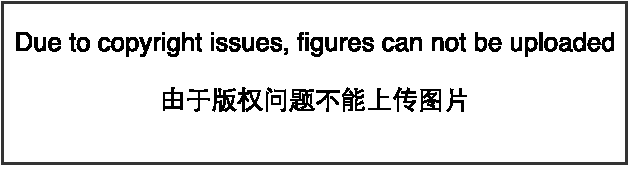
\includegraphics{figure.pdf}}
\else
\centerline{\includegraphics{Chapter7/figures/reg_l2}}
\fi
\caption{$L^2$(或\gls{weight_decay})\gls{regularization}对最佳的$\Vw$值的影响。
实线椭圆表示没有\gls{regularization}目标的等值线。
虚线圆圈表示$L^2$正则化项的等值线。
在$\tilde{\Vw}$点,这两个竞争目标达到平衡。
目标函数$J$的\gls{hessian}的第一维特征值很小。
当从$\Vw^*$水平移动时,\gls{objective_function}不会增加得太多。
因为\gls{objective_function}对这个方向没有强烈的偏好,所以正则化项对该轴具有强烈的影响。
正则化项将$w_1$拉向零。
而\gls{objective_function}对沿着第二维远离$\Vw^*$的移动非常敏感。
对应的特征值较大,表示高\gls{curvature}。
因此,\gls{weight_decay}对$w_2$的位置影响相对较小。
}
\label{fig:chap7_reg_l2}
\end{figure}

% -- 225 --

只有显著减小\gls{objective_function}方向的参数会被保留得相对完好。
无助于\gls{objective_function}减小的方向,即\gls{hessian}的小的特征值告诉我们,在这个方向的移动不会显著增加\gls{gradient}。
对应于这种不重要方向的分量会随训练过程中使用的\gls{regularization}而衰减掉。


目前为止,我们讨论了\gls{weight_decay}对优化一个抽象通用的二次\gls{cost_function}的影响。
这些影响怎么影响具体的机器学习?
我们可以研究\gls{linear_regression},其真实\gls{cost_function}是二次的,因此适合目前为止我们使用的分析。
再次应用分析,我们将能够获得相同结果的一个特例,但这次通过训练数据的术语表述。
\gls{linear_regression}的\gls{cost_function}是平方误差之和:
\begin{align}
 (\MX \Vw - \Vy)^\top (\MX \Vw - \Vy).
\end{align}
我们添加$L^2$正则项后,\gls{objective_function}变为
\begin{align}
  (\MX \Vw - \Vy)^\top (\MX \Vw - \Vy) + \frac{1}{2}\alpha \Vw^\top \Vw.
\end{align}
这会将普通方程的解从
\begin{align}
\label{eq:716w}
  \Vw = (\MX^\top \MX)^{-1} \MX^\top \Vy
\end{align}
变为
\begin{align}
\label{eq:717mw}
   \Vw = (\MX^\top \MX + \alpha \MI)^{-1} \MX^\top \Vy .
\end{align}
\eqnref{eq:716w}中的矩阵$\MX^\top\MX$与\gls{covariance}矩阵$\frac{1}{m}\MX^\top\MX$成正比。
$L^2$正则项将这个矩阵替换为\eqnref{eq:717mw}中的$ (\MX^\top \MX + \alpha \MI)^{-1}$
这个新矩阵与原来的是一样的,不同的仅仅是在对角加了$\alpha$。
这个矩阵的对角项对应于每个输入特征的\gls{variance}。
我们可以看到,$L^2$\gls{regularization}能让学习算法``感知''到具有较高方差的输入$\Vx$, 因此与输出目标的\gls{covariance}较小(相对增加方差)的特征的权重将会被收缩。

\subsection{$L^1$参数\glsentrytext{regularization}}
\label{sec:l1_regularization}
$L^2$\gls{weight_decay}是\gls{weight_decay}最常见的形式,还有其他的方法来惩罚模型参数的大小。
另一种选择是使用$L^1$\gls{regularization}。

对模型参数$\Vw$的$L^1$\gls{regularization}形式定义为:
\begin{align}
 \Omega(\Vtheta) = \norm{ \Vw }_1 = \sum_i | w_i |,
 \end{align}
即各个参数的绝对值之和\footnote{如同$L^2$\gls{regularization},我们能将参数\gls{regularization}其他非零值$\Vw^{(o)}$。在这种情况下,$L^1$\gls{regularization}将会引入不同的项$\Omega(\Vtheta)=
\|\Vw - \Vw^{(o)} \|_1 = \sum_i | w_i - w_i^{(o)} |$。}。
现在我们将讨论$L^1$\gls{regularization}对简单\gls{linear_regression}模型的影响, 与分析$L^2$\gls{regularization}时一样不考虑\gls{bias_aff}参数。  
我们尤其感兴趣的是找出$L^1$和$L^2$\gls{regularization}之间的差异。
与$L^2$\gls{weight_decay}类似,$L^1$\gls{weight_decay}的强度也可以通过缩放惩罚项$\Omega$的正超参数$\alpha$控制。 
因此,\gls{regularization}的\gls{objective_function}$\tilde{J}(\Vw;\MX, \Vy)$如下给出
\begin{align}
\tilde{J}(\Vw;\MX, \Vy) = \alpha \| \Vw \|_1 +  J(\Vw;\MX, \Vy) ,
\end{align}
对应的梯度(实际上是次梯度):
\begin{align}
\label{eq:subgradient}
  \nabla_{\Vw} \tilde{J}(\Vw; \MX, \Vy) = \alpha \text{sign}(\Vw) + \nabla_{\Vw} J(\Vw; \MX, \Vy), % ?? may be wrong
\end{align}
其中$\text{sign}(\Vw)$只是简单地取$\Vw$各个元素的符号。

% -- 227 --

观察\eqnref{eq:subgradient},我们立刻发现$L^1$的\gls{regularization}效果与$L^2$大不一样。
具体来说,我们可以看到\gls{regularization}对\gls{gradient}的贡献不再是线性地缩放每个$w_i$;而是用与$\text{sign}(w_i)$同号的常数因子。
这种形式的\gls{gradient}的一个后果是,我们不一定能得到$J(\MX, \Vy;\Vw)$二次近似的直接算术解($L^2$\gls{regularization}时可以)。 
 
我们可以通过\gls{taylor}级数表示\gls{cost_function}是二次的简单\gls{linear_model}。
或者我们可以设想,这是一个逼近更复杂模型的\gls{cost_function}的截断\gls{taylor}级数。
在这个设定下,\gls{gradient}由下式给出
\begin{align}
  \nabla_{\Vw} \hat{J}(\Vw) = \MH (\Vw - \Vw^*),
\end{align}
同样,$\MH$是$J$在$\Vw^*$处计算的\gls{hessian}矩阵(关于$\Vw$)。

由于$L^1$惩罚项在满的、一般的\gls{hessian}的情况下,无法得到直接干净的代数表达式,因此我们将进一步简化假设\gls{hessian}是对角的,即$\MH = \text{diag}([H_{1,1},\dots, H_{n,n}])$,其中每个$H_{i,i}>0$。
如果用于\gls{linear_regression}问题的数据已被预处理(如可以使用PCA),去除了输入特征之间的相关性,那么这一假设成立。

我们可以将$L^1$\gls{regularization}目标函数的二次近似分解成一个关于参数的求和:
\begin{align}
 \hat J(\Vw; \MX, \Vy) = J(\Vw^*; \MX, \Vy) + \sum_i \Bigg [\frac{1}{2} H_{i,i} (w_i - w_i^*)^2 
 + \alpha |w_i| \Bigg].  % I think this is correct
\end{align}
有解析解(对每一维$i$)可以最小化这个近似\gls{cost_function},如下列形式:
\begin{align}
w_i = \text{sign}(w_i^*) \max\Big\{ |w_i^*| - \frac{\alpha}{H_{i,i}} , 0\Big\} .
\end{align}
考虑所有$i$且$w_i^* > 0$的情形,会有两种可能输出:
\begin{enumerate}
\item $w_i^* \leq \frac{\alpha}{H_{i,i}}$的情况。
\gls{regularization}后的目标中$w_i$的最优值是$w_i = 0$。
这是因为在方向$i$上$J(\Vw; \MX, \Vy) $对于$ \hat J(\Vw; \MX, \Vy)$的贡献受到压制,$L^1$\gls{regularization}项将$w_i$推向0。
\item  $w_i^* > \frac{\alpha}{H_{i,i}}$的情况。在这种情况,\gls{regularization}不会将$w_i$的最优值移向0,而仅仅在那个方向移动$\frac{\alpha}{H_{i,i}}$的距离。
\end{enumerate}
$w_i^* < 0$的情况与之类似,但是$L^1$惩罚项使$w_i$更接近0(减少$ \frac{\alpha}{H_{i,i}}$)或者为0。

相比$L^2$\gls{regularization},$L^1$\gls{regularization}会产生更\firstgls{sparse}的解。
在此\gls{sparse}性指的是一些参数具有0的最优值。
$L^1$\gls{regularization}的\gls{sparse}性是相比$L^2$\gls{regularization}是质的不同。
\eqnref{eq:713L2}给出了$L^2$\gls{regularization}的解$\tilde \Vw$。 
如果我们使用$L^1$\gls{regularization}分析时\gls{hessian}$\MH$为对角正定的假设,重新考虑这个等式,我们发现
$\tilde{w_i} = \frac{H_{i,i}}{H_{i,i} + \alpha} w_i^*$。
如果$w_i^*$不是0,那$\tilde{w_i}$也会保持非0。 
这表明$L^2$\gls{regularization}不会导致参数变得\gls{sparse},而$L^1$\gls{regularization}有可能通过足够大的$\alpha$实现\gls{sparse}。
 
由$L^1$\gls{regularization}导出的\gls{sparse}性质已经被广泛地用作\firstgls{feature_selection}机制。
\gls{feature_selection}从可用的特征子集选择应该使用的子集,简化了\gls{ML}问题。
特别是著名的LASSO\citep{Tibshirani95}(Least Absolute Shrinkage and
Selection Operator)模型将$L^1$惩罚和\gls{linear_model}结合,并使用最小二乘\gls{cost_function}。 
$L^1$惩罚使部分子集的权重为零,表明相应的特征可以被安全地忽略。
 
在\secref{sec:maximum_a_posteriori_map_estimation},我们看到许多\gls{regularization}策略可以被解释为\glssymbol{MAP}贝叶斯推断,
 特别是$L^2$\gls{regularization}相当于权重是高斯先验的\glssymbol{MAP}贝叶斯推断。
 对于$L^1$\gls{regularization},
用于\gls{regularization}一个\gls{cost_function}的惩罚项$\alpha \Omega(\Vw) =  \alpha \sum_i |w_i |$与先验是各向同性拉普拉斯分布(\eqnref{eq:chap3_laplace})($\Vw \in \SetR^n$)的\glssymbol{MAP}贝叶斯推断的最大化对数先验项是等价的:
\begin{align}
\log p(\Vw) = \sum_i \log \text{Laplace}(w_i;0,\frac{1}{\alpha}) = 
  -\alpha \norm{\Vw}_1 + n \log \alpha - n \log 2.
\end{align}
因为是关于$\Vw$最大化进行学习,我们可以忽略$\log \alpha - \log 2$项,因为它们与$\Vw$无关。
 
 % -- 229 --
 
 \section{作为约束的范数惩罚}
 \label{sec:7.2}
考虑通过参数范数\gls{regularization}的\gls{cost_function}:
\begin{align}
 \tilde{J}(\Vtheta;\MX, \Vy) = J(\Vtheta;\MX, \Vy) + \alpha \Omega(\Vtheta) .
\end{align}

回顾\secref{sec:constrained_optimization}我们可以通过构造一个\gls{generalized_lagrange_function}来最小化受约束的函数,即在原始\gls{objective_function}加上一系列惩罚项。
每个惩罚是一个系数之间的乘积,称为\firstgls{KKT}乘子,以及一个表示约束是否满足的函数。
如果我们想约束$\Omega(\Vtheta)$小于某个常数$k$,我们可以构建\gls{generalized_lagrange_function}
\begin{align}
 \CalL(\Vtheta, \alpha; \MX, \Vy) = J(\Vtheta; \MX, \Vy) + \alpha (\Omega(\Vtheta) - k).
\end{align}

这个约束问题的解由下式给出
\begin{align}
 \Vtheta^* = \underset{\Vtheta}{ \argmin} \underset{\alpha, \alpha>0}{\max} \CalL(\Vtheta, \alpha).
\end{align}

如\secref{sec:constrained_optimization}中描述,解决这个问题需要同时改变$\Vtheta$和$\alpha$。
\secref{sec:example_linear_least_squares}给出了一个带$L^2$约束的\gls{linear_regression}实例。
许多不同的程序是可能的,有些可能会利用\gls{GD}而其他可能使用\gls{gradient}为0的解析解,但在所有程序中$\alpha$在$\Omega(\Vtheta) > k$时必须增加,在$\Omega(\Vtheta) < k$时必须减小。
所有正的$\alpha$鼓励$\Omega(\Vtheta)$收缩。
最佳值$\alpha^*$也将鼓励$\Omega(\Vtheta)$收缩,但不会如$\Omega(\Vtheta)$小于$k$时那么强烈。

为了洞察约束的影响,我们可以固定$\alpha^*$,把这个问题看成只跟$\Vtheta$有关的函数:
\begin{align}
 \Vtheta^* =  \underset{\Vtheta}{ \argmin} ~\CalL(\Vtheta, \alpha^*) = 
 \underset{\Vtheta}{ \argmin}~
 J(\Vtheta; \MX, \Vy) + \alpha^* \Omega(\Vtheta).
\end{align}
这和最小化$\tilde J$的\gls{regularization}训练问题是完全一样的。
因此,我们可以把参数范数惩罚看作对权重强加的约束。
如果$\Omega$是$L^2$范数,那么权重就是被约束在一个$L^2$球中。
如果$\Omega$是$L^1$范数,那么权重就是被约束在一个$L^1$范数限制的区域中。
通常我们不知道通过使用\gls{weight_decay}的系数$\alpha^*$约束的区域大小,因为$\alpha^*$的值不直接告诉我们$k$的值。
原则上可以解得$k$,但$k$和$\alpha^*$之间的关系取决于的$J$的形式。
虽然我们不知道约束区域的确切大小,但我们可以通过增加或者减小$\alpha$来大致扩大或收缩约束区域。
较大的$\alpha$,将导致一个较小的约束区域。
较小的$\alpha$,将导致一个较大的约束区域。

% -- 230 --

有时候,我们希望使用显式的限制,而不是惩罚。
如\secref{sec:constrained_optimization}所描述,我们能修改下降算法(如\gls{SGD}算法),使其先计算$J(\Vtheta)$的下降步,然后将$\Vtheta$投影到满足$\Omega(\Vtheta) < k$的最近点。
如果我们知道什么样的$k$是合适的,而不想花时间寻找对应于此$k$处的$\alpha$值,这会非常有用。

另一个使用显式约束和重投影而不是使用惩罚强加约束的原因是惩罚可能导致非凸优化程序而陷入局部极小(对应于小的$\Vtheta$)。
当训练\gls{NN},这通常表现为训练带有几个``死单元''的\gls{NN}。
这些单元不会对网络学到的函数的行为有太大贡献,因为进入或离开他们的权重都非常小。
当使用权重范数的惩罚训练,这些配置可以是局部最优,即使可能通过增加权重以显著减少$J$。
通过重投影实现的显式约束可以在这些情况下工作得更好,因为它们不鼓励权重接近原点。
通过重投影实现的显式约束只在权重变大并试图离开限制区域时产生作用。

最后,因为重投影的显式约束还对优化过程增加了一定的稳定性,因此是另一个好处。
当使用较高的学习率时,很可能进入的正反馈,即大的权重诱导大\gls{gradient},然后诱发权重的大更新。
如果这些更新持续增加权重的大小,$\Vtheta$就会迅速增大,直到离原点很远而发生溢出。
重投影的显式约束可以防止这种反馈环引起的权重无限制持续增加。
\cite{Hinton-et-al-arxiv2012}建议结合使用约束和高学习速率,能更快地参数空间探索,并保持一定的稳定性。

% -- 231 --

\cite{Hinton-et-al-arxiv2012}尤其推荐由\cite{Srebro05}引入的策略:约束\gls{NN}层的权重矩阵每列的范数,而不是限制整个权重矩阵的\ENNAME{Frobenius}范数。
分别限制每一列的范数可以防止某一\gls{hidden_unit}有非常大的权重。
如果我们将此约束转换成\ENNAME{Lagrange}函数中的一个惩罚,这将与$L^2$ \gls{weight_decay}类似但每个\gls{hidden_unit}的权重都具有单独的\glssymbol{KKT}乘子。
每个\glssymbol{KKT}乘子分别会被动态更新,以使每个\gls{hidden_unit} 服从约束。
在实践中,列范数的限制总是通过重投影的显式约束实现。

\section{\glsentrytext{regularization}和欠约束问题}
\label{sec:regularization_and_under_constrained_problems}
在某些情况下,为了正确定义\gls{ML}问题,\gls{regularization}是必要的。
\gls{ML}中许多\gls{linear_model},包括\gls{linear_regression}和PCA,都依赖于求逆矩阵$\MX^\top\MX$。
只要$\MX^\top\MX$是奇异的这就是不可能的。
每当数据生成分布的一些方向上真的没有差异时,或因为例子较少(即相对输入特征,$\MX$的列来说)而在一些方向没有观察到\gls{variance},这个矩阵都是奇异的。
在这种情况下,\gls{regularization}的许多形式对应于求逆$\MX^\top\MX + \alpha \MI$。
这个\gls{regularization}矩阵可以保证是可逆的。

相关矩阵可逆时,这些线性问题有封闭形式的解。
没有闭合形式解的问题也可能是欠定。
一个例子是应用于线性可分问题的\gls{logistic_regression}。
如果权重向量$\Vw$是能够实现完美分类,那么$2 \Vw$也以较高似然实现完美分类。
类似\gls{SGD}的迭代优化算法将持续增加$\Vw$的大小,理论上将永远不会停止。
在实践中,数值实现的\gls{GD}最终会达到导致数值溢出的超大权重,此时的行为将取决于程序员如何处理这些不是真正数字的值。

大多数形式的\gls{regularization}能够保证应用于欠定问题的迭代方法收敛。
例如,当似然的斜率等于\gls{weight_decay}的系数时, \gls{weight_decay}将导致\gls{GD}不再增加权重的大小。

使用\gls{regularization}来解决欠定问题的想法超出了\gls{ML}范畴。
同样的想法在几个基本线性代数问题中也非常有用。

% -- 232 --

正如我们在\secref{sec:the_moore_penrose_pseudoinverse}看到,我们可以使用\ENNAME{Moore-Penrose}求解欠定线性方程。 
回想$\MX$伪逆$\MX^+$的一个定义:
\begin{align} 
\label{eq:729pseudo}
 \MX^+ = \lim_{\alpha \searrow 0} (\MX^\top \MX + \alpha \MI)^{-1}\MX^\top.
\end{align}
现在我们可以将\secref{eq:729pseudo}看作执行具有\gls{weight_decay}的\gls{linear_regression}。
具体来说,当\gls{regularization}系数趋向0时,\eqnref{eq:729pseudo}是\eqnref{eq:717mw}的极限。
因此,我们可以将伪逆解释为使用\gls{regularization}来稳定欠定问题。


\section{数据集增强}
\label{sec:dataset_augmentation_chap7}
让\gls{ML}模型泛化得更好的最好办法是用更多的数据来训练。
当然,在实践中,我们拥有数据量是有限的。
解决这个问题的一种方法是创建假数据并把它添加到训练集。
对于一些\gls{ML}任务,创造新的假数据是相当简单。

对分类来说这种方法是最简单的。
<BAD>分类器需要一个复杂的高维输入$\Vx$,并用单一类别的身份$y$总结$\Vx$。
这意味着分类面临的一个主要任务是要对各种各样的变换保持不变。
我们可以轻易通过转换训练集中的$\Vx$来生成新的$(\Vx, y)$对。

这种方法对于其他许多任务来说并不那么容易。
例如,在一个密度估计任务中的产生新的假数据是困难的,除非我们已经解决了密度估计问题。

数据集增强对一个具体的分类问题来说是一个特别有效的方法:对象识别。
图像是高维的并包括各种巨大的变化因素,其中有许多可以容易地模拟。
即使模型已使用卷积和\gls{pooling}技术(\chapref{chap:convolutional_networks})对部分平移保持不变,沿训练图像每个方向平移几个像素的操作通常可以大大改善泛化。
许多其他操作如旋转图像或缩放图像也已被证明非常有效。

我们必须要小心,不能应用改变正确类别的转换。
例如,光学字符识别任务需要认识``b''和``d''以及``6''和``9''的区别,所以对这些任务来说,水平翻转和旋转$180^{\circ}$并不是适当的数据集增强方式。

% -- 233 --

能保持我们希望的分类不变,但不容易执行的转换也是存在的。
例如,平面外绕轴转动难以通过简单的几何运算在输入像素上实现。

数据集增强对语音识别任务也是有效的\citep{Jaitly_VTLP_2013}。

在\gls{NN}的输入层注入噪声\citep{SietsmaDow91}也可以被看作是数据增强的一种形式。
对于许多分类甚至一些回归任务,即使小的随机噪声被加到输入,任务仍应该是能解决的。
然而 ,\gls{NN}被证明对噪声不是非常健壮\citep{TangElias10}。
改善\gls{NN}健壮性的方法之一是简单地将随机噪声施加到其输入再进行训练。
输入噪声注入是一些无监督学习算法的一部分,如降噪\gls{AE}\citep{VincentPLarochelleH2008}。
当噪声被施加到\gls{hidden_unit}也是可行的,这可以被看作是在多个抽象层上进行的数据集增强。
\cite{Poole14}最近表明,噪声的幅度被细心调整后,该方法是非常高效的。
\gls{dropout},一个将在\secref{sec:dropout}描述的强大的\gls{regularization}策略,可以被看作是通过\emph{乘}噪声来构建新输入的过程。

当比较\gls{ML}基准测试的结果时,将其采取的数据集增强的影响考虑在内是很重要的。
通常情况下,人工设计的数据集增强方案可以大大减少\gls{ML}技术的泛化误差。
将一个\gls{ML}算法的性能与另一个进行对比时,对照实验是必要的。
当比较\gls{ML}算法A和\gls{ML}算法B时,应该确保这两个算法使用同一个人工设计的数据集增强方案进行评估。
假设算法A在没有数据集增强时表现不佳,而B结合大量人工转换的数据后表现良好。
在这样的情况下,很可能是合成转化引起了性能改进,而不是\gls{ML}算法B。 
有时候,确定实验是否已经适当控制需要主观判断。
例如,噪声注入输入的\gls{ML}算法是执行数据集增强的一种形式。
通常,普适操作(例如,向输入添加高斯噪声)被认为是\gls{ML}算法的一部分,
而特定于一个应用领域(如随机地裁剪图像)的操作被认为是独立的预处理步骤。

% -- 234 --

\section{噪声鲁棒性}
\label{sec:noise_robustness}

\secref{sec:dataset_augmentation_chap7}已经将噪声作用于输入的数据集增强策略。
对于某些模型,在模型的输入加上方差极小的噪音等价于对权重施加范数惩罚\citep{Bishop1995,bishop95training}。
在一般情况下,噪声注入远远比简单地收缩参数强大,特别是噪声被添加到\gls{hidden_unit}时。
向\gls{hidden_unit}添加噪音是值得单独讨论重要的话题;在\secref{sec:dropout}所述\gls{dropout}算法这种做法主要发展方向。

另一种\gls{regularization}模型的噪声使用方式是将其加到的权重。
这项技术主要被用于\gls{RNN}的情况下\citep{JimGilesHorne1996,Graves-2011}。
这可以解释为一个关于权重的贝叶斯\gls{inference}的随机实现。
使用贝叶斯处理学习过程将权重视为不确定的,且能通过概率分布表示的这种不确定性。
向权重添加噪声是反映这种不确定的一种实用的随机方法。

在某些假设下,施加于权重的噪声可以被解释为与更传统\gls{regularization}形式等同,鼓励要学习函数的稳定性。
我们研究回归的情形,也就是训练一个将一组特征$\Vx$映射成一个标量的函数$\hat y(\Vx)$,并使用最小二乘\gls{cost_function}衡量模型预测值$\hat y(\Vx)$与真实值$y$的误差:
\begin{align}
 J = \SetE_{p(x,y)}[(\hat y(\Vx) - y)^2].
\end{align}
训练集包含$m$对标注样例$\{(\Vx^{(1)}, y^{(1)}),\dots,(\Vx^{(m)}, y^{(m)})\}$

现在我们假设我们在对每个输入表示上添加网络权重的随机扰动$\epsilon_{\Vw} \sim \CalN(\Vepsilon;0, \eta\MI )$
想象我们有一个标准的$l$层MLP。
我们将扰动模型记为$\hat y_{\epsilon_{\MW}} (\Vx)$。
尽管有噪声的注入,我们仍对减少网络输出误差的平方感兴趣。
因此目标函数变为:
\begin{align}
 \tilde J_{\MW} &= \SetE_{p(\Vx,y,\epsilon_{\MW})}[(\hat y_{\epsilon_{\MW}}(\Vx) - y)^2] \\
   &=  \SetE_{p(\Vx,y,\epsilon_{\MW})}[\hat y_{\epsilon_{\MW}}^2(\Vx) -  2y\hat y_{\epsilon_{\MW}}
   (\Vx)+ y^2] .
\end{align}

对于小的$\eta$,最小化带权重噪声(方差为$\eta \MI$)的$J$等同于最小化附加上\gls{regularization}项的$J$:
$ \eta \SetE_{p(\Vx,y)}[\norm{\nabla_{\MW}~\hat y(\Vx)}^2]$。
这种形式的\gls{regularization}鼓励参数进入权重小扰动对输出相对影响较小的参数空间区域。
换句话说,它推动模型进入对权重小的变化相对不敏感的区域,找到的点不只是极小点,还是由平坦区域所包围的最小点\citep{Hochreiter95}。
在简化的线性回归(例如,$\hat y(\Vx) = \Vw^\top \Vx + b$),正则项退化为$ \eta \SetE_{p(\Vx)}[\norm{\Vx}^2]$,这与
函数的参数无关,因此不会对$\tilde J_{\Vw}$关于模型参数的梯度有贡献。

% -- 235 --

\subsection{向输出目标注入噪声}
\label{sec:injecting_noise_at_the_output_targets}
大多数数据集的$y$标签都有一定错误。
当$y$是错误的,那对最大化$\log p(y \mid \Vx)$会是有害的。
为了防止这一点的一种方法是显式地对标签上的噪声进行建模。
例如,我们可以假设,对于一些小常数$\epsilon$,训练集标记$y$是正确的概率是$1-\epsilon$,任何其他可能的标签可能是正确的。
这个假设很容易就能解析地与\gls{cost_function}结合,而不用显式地采噪声样本。
例如, \textbf{标签平滑}(label smoothing)基于$k$个输出的\gls{softmax},把明确分类0和1替换成$\frac{\epsilon}{k-1}$和$1-\epsilon$,对模型进行\gls{regularization}。
标准交叉熵损失可以用在这些非确切目标的输出上。
使用\gls{softmax}和明确目标的最大似然学习可能永远不会收敛——
\gls{softmax}永远无法真正预测0概率或1概率,因此它会继续学习越来越大的权重,使预测更极端。
使用如\gls{weight_decay}等其他\gls{regularization}策略能够防止这种情况。
标签平滑的优势是能防止模型追求明确概率而不妨碍正确分类。
这种策略自20世纪80年代就已经被使用,并在现代神经网络继续保持显著特色\citep{Szegedy-et-al-2015}。

% -- 236 --

\section{半监督学习}
\label{sec:semi_supervised_learning}
在半监督学习的框架下,$P(\RVx)$产生的未标记样本和$P(\RVx, \RVy)$中的标记样本都用于估计$P(\RVy \mid \RVx)$或者根据$\RVx$预测$\RVy$。

在\gls{DL}的背景下,半监督学习通常指的是学习一个\gls{representation}$h = f(\Vx)$。 
学习\gls{representation}的目标是使相同类中的\gls{example}有类似的表示。
无监督学习可以为如何在\gls{representation}空间聚集\gls{example}提供有用的线索。
在输入空间紧密聚集的\gls{example}应该被映射到类似的表示。
在新空间上的线性分类器在许多情况下可以达到较好的泛化\citep{Belkin+Niyogi-2002,Chapelle+al-2003}。
这种方法的长期存在的一个变种是应用主成分分析作为分类前(在投影后的数据上分类)的预处理步骤。

我们可以构建一个模型,其中生成模型$P(\RVx)$或$P(\RVx, \RVy)$与判别模型$P(\RVy \mid \RVx)$共享参数,而不用将无监督和监督部分分离。
可以对监督\gls{criterion}$-\log P(\Vy \mid \Vx)$与无监督或生成的\gls{criterion}(如$-\log P(\Vx)$或$-\log P(\Vx, \Vy)$)进行权衡。
生成模型\gls{criterion}表达了对监督学习问题解的特殊形式的先验知识\citep{LasserreJ2006},即$P(\RVx)$的结构通过某种共享参数的方式连接到$P(\RVy \mid \RVx)$。
通过控制在总\gls{criterion}中的生成\gls{criterion},我们可以找到比纯生成或纯判别训练\gls{criterion}更好的权衡\citep{LasserreJ2006,Larochelle2008}。

\cite{Russ+Geoff-nips-2007}描述了一种学习回归内核机中内核函数的方法,其中建模的$P(\RVx)$时使用的未标记的样本大大提高了$P(\RVy \mid \RVx)$。

更多半监督学习的信息,请参阅\cite{SSL-Book-2006}。

\section{多任务学习}
\label{sec:multitask_learning}
多任务学习\citep{caruana93a}是通过合并几个任务中的样例(可以视为对参数施加的软约束)来提高泛化的一种方式。
额外的训练样本以同样的方式将模型的参数推向泛化更好的方向,当模型的一部分在任务之间共享时,模型的这一部分被更多地约束为良好的值(假设共享是合理的),往往能更好的泛化。

\figref{fig:chap7_multi_factor_output}展示了多任务学习中非常普遍的一种形式,其中不同的监督任务(给定$\RVx$预测$\RVy^{(i)}$)共享相同的输入$\RVx$以及一些中间层表示$\Vh^{(\text{share})}$,能学习共同的因素池。
该模型通常可以分为两个部分和相关参数:
\begin{enumerate}
 \item 具体任务的参数 (只能从各自任务的样本中实现良好的泛化)。如\figref{fig:chap7_multi_factor_output}中的上层。
 \item 所有任务共享的通用参数(从所有任务的汇集数据中获益)。如\figref{fig:chap7_multi_factor_output}中的下层。
\end{enumerate}
\begin{figure}[!htb]
\ifOpenSource
\centerline{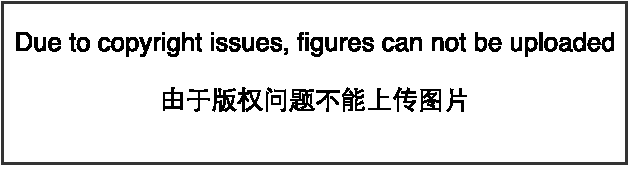
\includegraphics{figure.pdf}}
\else
\centerline{\includegraphics{Chapter7/figures/multi_factor_output}}
\fi
\caption{TODO}
\label{fig:chap7_multi_factor_output}
\end{figure}

因为共享参数,其统计强度可大大提高(共享参数的样本数量相对于单任务模式增加的比例),能改善泛化和泛化误差的范围\citep{baxter95a}。
当然,仅当不同的任务之间存在某些统计关系的假设是合理时才会发生,也就是意味着某些参数能通过不同任务共享。

从\gls{DL}的观点看,底层的先验知识如下:\emph{能解释数据变化(在与之相关联的不同任务中观察到)的因素中,一些是跨两个或更多任务共享的。}

% -- 238 --

\section{\glsentrytext{early_stopping}}
\label{sec:early_stopping}
当训练有足够的表示能力甚至会过度拟合的大模型时,我们经常观察到,训练误差会随着时间的推移逐渐降低但验证集的误差会再次上升。
\figref{fig:chap7_learning_curve}是这些现象的一个例子,这种现象几乎一定会出现。

这意味着我们可以返回使验证集误差最低的参数设置来获得更好的模型(因此,有希望获得更好的测试误差)。
在每次验证集误差有所改善后,我们存储模型参数的副本。
当训练算法终止时,我们返回这些参数而不是最新的参数。
当验证集上的误差在事先指定的循环内没有进一步改善时,算法就会终止。
此过程在算法|||c|||有更正式的说明。

% -- 239 --

这种策略被称为\firstgls{early_stopping}。
这可能是\gls{DL}中最常用的\gls{regularization}形式。
它的流行主要是因为有效性和简单性。

\begin{figure}[!htb]
\ifOpenSource
\centerline{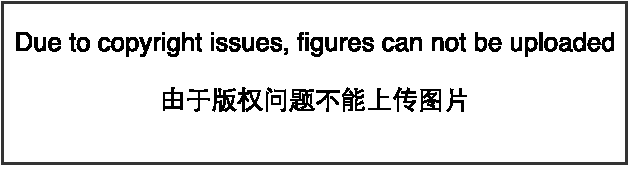
\includegraphics{figure.pdf}}
\else
\centerline{\includegraphics{Chapter7/figures/learning_curve_color}}
\fi
\caption{TODO}
\label{fig:chap7_learning_curve}
\end{figure}

我们可以认为\gls{early_stopping}是非常高效的超参数选择算法。
按照这种观点,训练步数仅是另一个超参数。
我们从\figref{fig:chap7_learning_curve}可以看到的,这个超参数在验证集上的具有U形性能曲线。
很多控制模型容量的超参数在验证集上都是这样的U型性能曲线,如\figref{fig:chap7_learning_curve}。
在\gls{early_stopping}的情况下,我们通过拟合训练集的步数来控制模型的有效容量。
大多数超参数的选择必须使用昂贵的猜测和检查过程,我们需要在训练开始时猜测一个超参数,然后运行几个步骤检查它的训练效果。
``训练时间''唯一只要跑一次训练就能尝试很多值的超参数。
通过\gls{early_stopping}自动选择超参数的唯一显著的代价是训练期间要定期评估验证集。
理想情况下,这是可以并行在与主训练过程分离的机器,或独立的CPU,或独离的GPU上完成。
如果没有这些额外的资源,可以使用比训练集小的验证集或较不频繁地评估验证集来减小评估代价,较粗略地估算取得最佳的训练时间。

另一个\gls{early_stopping}的额外代价是需要保持最佳的参数副本。
这种代价一般是可忽略的,因为将它储存在较慢的较大的存储器上,(例如,在GPU内存中训练,但将最佳参数存储在主存储器或磁盘驱动器上)。
由于最佳参数的写入很少发生而且从不在训练过程中读取,这些偶发的慢写入对总训练时间的影响不大。

% -- 240 --

\gls{early_stopping}是\gls{regularization}的非常不显眼的形式,它几乎不需要对基本训练过程、\gls{objective_function}或一组允许的参数值进行变化。
这意味着,无需破坏学习动态就能很容易地使用\gls{early_stopping}。
相对于\gls{weight_decay},必须小心不能使用太多的\gls{weight_decay},防止网络陷入不良\gls{local_minimum}(对应于病态的小权重)。

\gls{early_stopping}可单独使用或与其它的\gls{regularization}策略相结合。
即使修改\gls{objective_function}以鼓励更好泛化的\gls{regularization}策略,在训练目标的\gls{local_minimum}达到最好泛化也是非常罕见的。

\gls{early_stopping}需要验证集,这意味着某些训练数据不能被馈送到模型。
为了更好地利用这一额外的数据,我们可以使用\gls{early_stopping}初步训练之后,进行额外的训练。
在第二轮额外的训练步骤中,所有的训练数据都被包括在内。
有两个基本的策略可以用于第二轮训练过程。

% -- 241 --

一种策略(算法|||c|||)是再次初始化模型,然后使用所有数据再次训练。
在这个第二轮训练过程,我们使用第一轮\gls{early_stopping}训练确定的最佳步数。
此过程有一些细微之处。
例如,我们没有办法知道重新训练时对参数进行相同次数的更新和对数据集进行相同的遍数哪一个更好。
由于训练集变大了,在第二轮训练时,每遍历一次数据集将会对应更多次的参数更新。

另一个策略是保持从第一轮训练获得的参数,然后使用全部的数据\emph{继续}训练。
在这个阶段中,现在我们已经在训练多少步停止上不再有指导。
相反,我们可以监控验证集的平均损失函数,并继续训练,直到它低于\gls{early_stopping}过程停止时的目标值。
此策略避免了重新训练模型的高成本,但表现并没有那么好。
例如,验证集的目标不一定能达到之前的目标值,所以这种策略甚至不能保证终止。
这个过程在算法|||c|||中更正式地展示。

\gls{early_stopping}对减少训练过程的计算成本也是有用的。
除了由于限制训练的迭代次数而明显减少的计算成本,还带来了\gls{regularization}的益处(不需要添加惩罚项的\gls{cost_function}或计算这种附加项的\gls{gradient})。

% -- 242 --

\paragraph{\gls{early_stopping}是如何充当\gls{regularization}的:}
目前为止,我们已经声明\gls{early_stopping}是一种\gls{regularization} 策略,但我们只通过展示验证集误差的学习曲线是一个U形的来支持这种说法。
\gls{early_stopping}\gls{regularization}模型的真正机制是什么? 
\cite{Bishop1995}和\cite{Sjoberg95}认为\gls{early_stopping}具有将优化过程的参数空间限制在初始参数值$\Vtheta_0$相对小的邻域内的效果。
更具体地,想象用学习率$\epsilon$进行$\tau$个优化步骤(对应于$\tau$个训练迭代)。
我们可以将$\epsilon \tau$作为有效容量的度量。
假设\gls{gradient}有界,限制迭代的次数和学习速率会限制从$\Vtheta_0$到达的参数空间大小,如\figref{fig:chap7_reg_l1_vs_l2_mistake}所示。
在这个意义上,$\epsilon \tau$的行为就好像它是\gls{weight_decay}系数的倒数。

\begin{figure}[!htb]
\ifOpenSource
\centerline{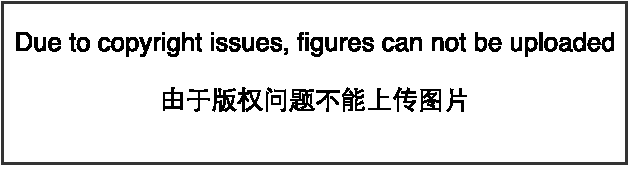
\includegraphics{figure.pdf}}
\else
\centerline{\includegraphics[width=0.8\textwidth]{Chapter7/figures/reg_l1_vs_l2_mistake}}
\fi
\caption{TODO}
\label{fig:chap7_reg_l1_vs_l2_mistake}
\end{figure}

事实上,在二次误差的简单\gls{linear_model}和简单的\gls{GD}情况下,我们可以展示\gls{early_stopping}相当于$L^2$\gls{regularization} 。

为了与经典$L^2$\gls{regularization}比较,我们考察唯一的参数是线性权重($\Vtheta = \Vw$)的简单设定。
我们在权重$\Vw$的经验最佳值$\Vw^*$附近以二次近似建模\gls{cost_function} $J$:
\begin{align}
 \hat J(\Vtheta) = J(\Vw^*) + \frac{1}{2}  (\Vw- \Vw^*)^\top \MH  (\Vw - \Vw^*),
\end{align}
其中$\MH$是$J$关于$\Vw$在$\Vw^*$点的\gls{hessian}。
鉴于假设$\Vw^*$是$J(\Vw)$的最小点,我们知道$\MH$为半正定。
在局部\gls{taylor}级数逼近下,\gls{gradient}由下式给出:
\begin{align}
 \nabla_{\Vw} \hat J (\Vw) = \MH (\Vw - \Vw^*).
\end{align}

% -- 243 --

我们要研究训练时参数向量的轨迹。
为简化起见,我们参数向量初始化为原点\footnote{对于\gls{NN},我们需要打破\gls{hidden_unit}间的对称平衡因此不能将所有参数都初始化为$\mathbf{0}$(如\secref{sec:gradient_based_learning}所讨论的)。
然而,对于其他任何初始值$\Vw_{(0)}$该论证都成立},也就是$\Vw^{(0)} = 0$。
我们通过分析$\hat{J}$的\gls{GD}研究$J$上近似的\gls{GD}行为:
\begin{align}
\Vw^{(\tau)} &= \Vw^{(\tau-1)} -\epsilon \nabla_{\Vw} \hat{J}( \Vw^{(\tau-1)} ) \\
&=  \Vw^{(\tau-1)}  - \epsilon  \MH ( \Vw^{(\tau-1)} -  \Vw^* ), \\
\Vw^{(\tau)}  -  \Vw^* &= (\MI - \epsilon  \MH) ( \Vw^{(\tau-1)} -  \Vw^* ).
 \end{align}
现在让我们在$\MH$特征向量的空间中改写表达式,利用$\MH$的特征分解:$\MH = \MQ \VLambda \MQ^\top$,其中$\VLambda$是对角矩阵,$\MQ$是特征向量的一组正交基。
\begin{align}
\Vw^{(\tau)}  -  \Vw^* &= (\MI - \epsilon \MQ \VLambda \MQ^\top) ( \Vw^{(\tau-1)} -  \Vw^* ) \\
\MQ^\top (\Vw^{(\tau)}  -  \Vw^*) &= (\MI - \epsilon \VLambda)\MQ^\top ( \Vw^{(\tau-1)} -  \Vw^* )
\end{align}
假定$\Vw^{(0)} = 0$并且$\epsilon$选择得足够小以保证$|1 - \epsilon \lambda_i |<1$,经过$\tau$次参数更新后轨迹如下:
\begin{align} \label{eq:740qw}
\MQ^\top  \Vw^{(\tau)} = [\MI - (\MI - \epsilon \VLambda)^\tau] \MQ^\top  \Vw^* .
\end{align}
现在,\eqnref{eq:713L2}中$\MQ^\top \tilde \Vw$的表达式能被重写为:
\begin{align}
\MQ^\top  \tilde \Vw &= (\VLambda + \alpha \MI)^{-1} \VLambda \MQ^\top  \Vw^*, \\
\MQ^\top  \tilde \Vw &= [\MI - (\VLambda + \alpha \MI)^{-1} \alpha] \MQ^\top  \Vw^*. 
\label{eq:742qw}
\end{align}
比较\eqnref{eq:740qw}和\eqnref{eq:742qw},我们能够发现,如果超参数$\epsilon,\alpha$和$\tau$满足如下:
\begin{align}
(\MI - \epsilon \VLambda)^\tau =  (\VLambda + \alpha \MI)^{-1} \alpha,
\end{align}\
那么$L^2$\gls{regularization}和\gls{weight_decay}可以被看作是等价的(至少在\gls{objective_function}的二次近似下)。
进一步取对数,使用$\log~(1+x)$的级数展开,我们可以得出结论,如果所有$\lambda_i$是小的(即$\epsilon \lambda_i \ll 1$且$\lambda_i / \alpha \ll 1$),那么
\begin{align}
\tau \approx \frac{1}{\epsilon \alpha}, \\
\alpha \approx \frac{1}{\tau \epsilon}.
\end{align}
也就是说,在这些假设下,训练迭代次数$\tau$起着与$L^2$参数成反比的作用,$\tau \epsilon$的倒数与\gls{weight_decay}系数的作用类似。

对应显著曲率(\gls{objective_function})方向的参数值\gls{regularization}小于小曲率方向。
当然,在\gls{early_stopping}的情况下,这实际上意味着对应于显著曲率方向的参数比较小的曲率方向的参数学习得更早。
 
本节中的推导表明长度为$\tau$的轨迹结束于最小的$L^2$\gls{regularization} 目标的最小点。
当然,\gls{early_stopping}比仅仅的轨迹长度限制更丰富;相反,\gls{early_stopping}通常涉及监控验证集的错误,以便在空间特别好的点处停止轨迹。
因此\gls{early_stopping}比\gls{weight_decay}更具有优势,\gls{early_stopping}能自动确定\gls{regularization}的正确量,而\gls{weight_decay}需要多个训练实验来测试其超参数的不同值。

% -- 245 --

\section{参数绑定和参数共享}
\label{sec:parameter_tying_and_parameter_sharing}
目前为止,本章讨论对参数添加约束或惩罚时,一直是相对于固定的区域或点。
例如,$L^2$\gls{regularization}(或\gls{weight_decay})对参数偏离零的固定值进行惩罚。
然而,有时我们可能需要其他的方式来表达我们对模型参数适当值的先验知识。
有时候,我们可能无法准确地知道应该采取什么样的参数,但我们从领域和模型结构方面的知识知道,模型参数之间应该存在一些相关性。

我们经常想要表达的常见类型的依赖是某些参数应当彼此接近。
考虑以下情形:我们有两个模型执行相同的分类任务(具有相同类别),但输入分布稍有不同。
形式地,我们有参数为$\Vw^{(A)}$的模型A和参数为$\Vw^{(B)}$的模型B。
这两种模型将输入映射到两个不同但相关的输出:$\hat y^{(A)} = f(\Vw^{(A)}, \Vx)$和$\hat y^{(B)} = f(\Vw^{(B)}, \Vx)$。

我们可以想象,这些任务是足够相似(或许具有相似的输入和输出分布),因此我们认为模型参数应彼此靠近:
$\forall i, w_i^{(A)}$应该与$ w_i^{(B)}$接近。
我们可以通过\gls{regularization}利用此信息。
具体来说,我们可以使用以下形式的参数范数惩罚:
$\Omega(\Vw^{(A)}, \Vw^{(B)}) = \norm{\Vw^{(A)}-\Vw^{(B)}}_2^2$。
在这里我们使用$L^2$惩罚,但也可以有其它选择。

这种方法由\cite{LasserreJ2006}提出,\gls{regularization}一个模型(监督模式下训练的分类器)的参数接近另一个无监督模式下训练的模型(捕捉观察到的输入数据的分布)。
这个架构的构造成使得许多分类模型中的参数能与对应的无监督模型的参数匹配。

参数范数惩罚是\gls{regularization}参数彼此接近的一种方式,在更流行的方法是使用约束:强迫某些集合中的参数相等。
由于我们将各种模型或模型组件解释为共享唯一的一组参数,这种\gls{regularization}方法通常被称为\firstgls{parameter_sharing}。
\gls{parameter_sharing}相对于\gls{regularization}参数接近(通过范数惩罚)的一个显著优点是,只有参数(唯一一个集合)的子集需要被存储在内存中。
对于某些特定模型,如\gls{CNN},这可能导致内存占用的显著减少。


% -- 246 --
\subsection{\glsentrytext{CNN}}
目前为止,最流行和广泛使用的\gls{parameter_sharing}出现在应用于\gls{CV}的\firstacr{CNN}。
自然图像有许多统计属性是对转换不变的。
例如,猫的照片即使向右边移了一个像素,仍保持猫的相片,。
\glssymbol{CNN}通过在图像多个位置共享参数考虑这个特性。
相同的特征(具有相同权重的\gls{hidden_unit})在输入的不同位置上计算。
这意味着无论猫出现在图像中的第$i$列或$i + 1$列,我们都可以使用相同的猫探测器找到猫。

\gls{parameter_sharing}显著降低\glssymbol{CNN}模型不同参数的数量,并显著提高了网络的大小而不需要增加相应的训练数据。
它仍然是将领域知识有效地整合到网络架构的最佳范例之一。

\gls{CNN}将会在\chapref{chap:convolutional_networks}更详细地讨论。

\section{\glsentrytext{sparse}\glsentrytext{representation}}
\label{sec:sparse_representations}
\gls{weight_decay}施加直接作用于模型参数的惩罚。
另一种策略是将惩罚放在\gls{NN}的激活单元,鼓励对应的激活是\gls{sparse}。
这间接的对模型参数施加了复杂惩罚。

我们已经讨论过(在\secref{sec:l1_regularization})$L^1$惩罚如何诱导\gls{sparse}的参数,意味着许多参数为零(或接近于零)。
\gls{representation}的\gls{sparse},在另一方面描述了一种其中许多的元素是零(或接近零)的\gls{representation}。
可以\gls{linear_regression}情况下简单说明这种区别:
\begin{align}
\underset{\Vy ~\in~ \SetR^m}{
 \begin{bmatrix}
  18 \\  5 \\ 15 \\ -9 \\ -3
 \end{bmatrix}} = 
 \underset{\MA ~\in~ \SetR^{m \times n}}{
 \begin{bmatrix}
  4 & 0 & 0 & -2 & 0 & 0 \\
  0 & 0 & -1 & 0 & 3 & 0 \\
  0 & 5 & 0 & 0 & 0 & 0 \\
  1 & 0 & 0 & -1 & 0 & -4 \\
  1 & 0 & 0 & 0 & -5 & 0
 \end{bmatrix}} 
  \underset{\Vx ~\in~ \SetR^n}{
  \begin{bmatrix}
 2 \\ 3\\ -2\\ -5 \\ 1 \\ 4
 \end{bmatrix} }\\
 \underset{\Vy ~\in~ \SetR^m}{
 \begin{bmatrix}
  -14 \\  1 \\ 19 \\  2 \\ 23
 \end{bmatrix}} = 
 \underset{\MB ~\in~ \SetR^{m \times n}}{
 \begin{bmatrix}
  3 & -1 & 2 & -5 & 4 & 1 \\
  4 & 2 & -3 & -1 & 1 & 3 \\
  -1 & 5 & 4 & 2 & -3 & -2 \\
  3 & 1 & 2 & -3 & 0 & -3 \\
  -5 & 4 & -2 & 2 & -5 & -1
 \end{bmatrix}} 
  \underset{\Vh \in \SetR^n}{
  \begin{bmatrix}
 0 \\ 2 \\ 0 \\ 0 \\ -3 \\ 0
 \end{bmatrix} }
\end{align}

% -- 247 --

第一个表达式是参数\gls{sparse}的\gls{linear_regression}模型的例子。
第二个是数据$\Vx$具有\gls{sparse}\gls{representation}$\Vh$的线性回归。
也就是说,$\Vh$是$\Vx$的一个函数,在某种意义上\gls{representation}存在于$\Vx$中的信息,但是用一个\gls{sparse}向量\gls{representation}。

\gls{representation}的\gls{regularization}可以通过在参数\gls{regularization}中使用的同种类型的机制来实现的。

\gls{representation}的范数惩罚\gls{regularization}是通过向\gls{loss_function}$J$添加对\gls{representation}的范数惩罚。
记这个惩罚为$\Omega(\Vh)$。
和以前一样,我们将\gls{regularization}后的损失函数记为$\tilde J$:
\begin{align}
 \tilde J(\Vtheta; \MX, \Vy) =  J(\Vtheta; \MX, \Vy)  + \alpha \Omega(\Vh),
\end{align}
其中$\alpha \in [0, \infty]$ 权衡范数惩罚项的相对贡献,越大的$\alpha$对应更多的\gls{regularization}。

正如对参数的$L^1$惩罚诱导参数\gls{sparse}性,对\gls{representation}元素的$L^1$惩罚诱导\gls{sparse}的\gls{representation}:
$\Omega(\Vh) = \norm{\Vh}_1 = \sum_i |h_i|$。
当然$L^1$惩罚是导致\gls{sparse}\gls{representation}的选择之一。
其他包括从\gls{representation}上\ENNAME{Student} $t$先验导出的惩罚\citep{Olshausen+Field-1996,Bergstra-Phd-2011}和\gls{KL}惩罚\citep{Larochelle+Bengio-2008}有利于表示元素约束于单位区间上。
<BAD>\cite{HonglakL2008-small}和\cite{Goodfellow2009}都提供了基于平均几个实例激活的\gls{regularization}策略的例子,$\sum_i^m \Vh^{(i)}$,使其接近某些目标值,如每项都是$.01$的向量。

其他的方法使用激活值的硬性约束获得\gls{representation}\gls{sparse}。
例如,\textbf{正交匹配追踪}(orthogonal matching pursuit)\citep{pati93orthogonal}通过解决\gls{constrained_optimization}问题将输入值$\Vx$编码成\gls{representation}$\Vh$
\begin{align}
 \underset{\Vh, \norm{\Vh}_0 < k}{\argmin} \norm{\Vx - \MW \Vh}^2,
\end{align}
其中$\norm{\Vh}_0 $是$\Vh$中非零项的个数。
当$\MW$被约束为正交时,这个问题可以高效地解决。
这种方法通常被称为\ENNAME{OMP-k},通过$k$指定允许非零特征的数量。
\cite{Coates2011b}证明\ENNAME{OMP-1}可以成为深度架构中非常有效的特征提取器。

% -- 248 --

有\gls{hidden_unit}的模型本质上都能变得\gls{sparse}。
在这本书中,我们将看到各种情况下使用\gls{sparse}\gls{regularization}的例子。

\section{\glsentrytext{bagging}和其他\glsentrytext{ensemble}的方法}
\label{sec:bagging_and_other_ensemble_methods}
\firstgls{bagging}是通过结合几个模型降低泛化误差的技术\citep{ML:Breiman:bagging}。
主要想法是分别训练几个不同的模型,然后让所有模型表决测试样例的输出。
这在\gls{ML}中普通策略的一个例子,被称为\firstgls{model_averaging}。
采用这种策略的技术被称为\gls{ensemble}方法。

\firstgls{model_averaging}奏效的原因是不同的模型通常不会在测试集上产生完全相同的错误。

考虑$k$个回归模型的例子。
假设每个模型在每个例子上的误差是$\epsilon_i$,这个误差服从零均值\gls{variance}为$\SetE[\epsilon_i^2] = v$且\gls{covariance}为$\SetE[\epsilon_i \epsilon_j] = c$的多维正态分布。
通过所有\gls{ensemble}模型的平均预测所得误差是$\frac{1}{k} \sum_i \epsilon_i$。 
\gls{ensemble}预测器平方误差的期望是
\begin{align}
 \SetE \Bigg[\Bigg(\frac{1}{k} \sum_i \epsilon_i \Bigg)^2\Bigg] &= \frac{1}{k^2} 
 \SetE \Bigg[\sum_i \Bigg(\epsilon_i^2 + \sum_{j \neq i} \epsilon_i \epsilon_j\Bigg)\Bigg], \\
&= \frac{1}{k} v + \frac{k-1}{k} c .                             
\end{align}
在误差完全相关即$c=v$的情况下,均方误差减少到$v$,所以\gls{model_averaging}没有任何帮助。
在错误完全不相关即$c =0$的情况下,该\gls{ensemble}平方误差的期望仅为$\frac{1}{k}v$。
这意味着\gls{ensemble}平方误差的期望会随着\gls{ensemble}的大小线性地减小。
换言之,\gls{ensemble}平均上至少与它的任何成员表现得一样好,并且如果成员的误差是独立的,\gls{ensemble}将显著地比其成员表现得更好。

不同的\gls{ensemble}方法以不同的方式构建\gls{ensemble}模型。
例如,\gls{ensemble}的每个成员可以使用不同的算法和\gls{objective_function}训练成完全不同的模型。
\gls{bagging}是一种允许重复多次使用同一种模型、训练算法和\gls{objective_function}的方法。

% -- 249 --

具体来说,\gls{bagging}涉及构造$k$个不同的数据集。
每个数据集与原始数据集具有相同数量的样例,但从原始数据集中有替换采样构成。
这意味着,每个数据集以高概率缺少一些来自原始数据集的例子,还包含若干重复的例子(如果所得训练集与原始数据集大小相同,那所得数据集中大概有原始数据集$2/3$的实例)。
模型$i$在数据集$i$上训练。
每个数据集包含样本的差异导致训练模型之间的差异。
\figref{fig:chap7_bagging}是一个例子。

\begin{figure}[!htb]
\ifOpenSource
\centerline{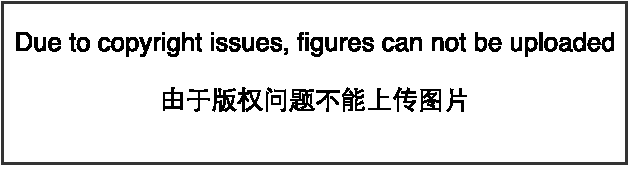
\includegraphics{figure.pdf}}
\else
\centerline{\includegraphics{Chapter7/figures/bagging}}
\fi
\caption{TODO}
\label{fig:chap7_bagging}
\end{figure}

\gls{NN}的解能达到足够多的变化意味着他们可以从\gls{model_averaging}中受益(即使所有模型都在同一数据集上训练)。
\gls{NN}中随机初始化的差异、\gls{minibatch}的随机选择、超参数的差异或不同输出的非确定性的实现往往足以引起\gls{ensemble}中不同成员的误差部分独立。

% -- 250 --

\gls{model_averaging}是减少泛化误差一个非常强大可靠的方法。
作为科学论文算法的基准时,它通常是不鼓励使用的,因为任何\gls{ML}算法可从\gls{model_averaging}中大幅获益(以增加计算和存储的代价)。

\gls{ML}比赛通常使用超过几十种\gls{model_averaging}的方法取胜。
最近一个突出的例子是\ENNAME{Netflix Grand Prize}\citep{Koren09}。

不是所有构建\gls{ensemble}的技术都是为了让\gls{ensemble}模型比单一模型更加\gls{regularization}。
例如,一种被称为\firstgls{boosting}的技术\citep{ConfLT:Freund:gametheorie,ConfML:Freund:AdaBoostCompar}构建比单一模型容量更高\gls{ensemble}模型。
向\gls{ensemble}逐步添加\gls{NN},\gls{boosting}已经应用于构建神经网络的\gls{ensemble}\citep{Schwenk-nips10}。
\gls{boosting}也可以将单个神经网络解释为单个\gls{ensemble},即通过逐渐增加\gls{NN}的\gls{hidden_unit}。

\section{\glsentrytext{dropout}}
\label{sec:dropout}
\firstgls{dropout}\citep{Srivastava14}提供了\gls{regularization}一大类模型的方法,计算方便但功能强大的。
第一个近似下,\gls{dropout}可以被认为是\gls{ensemble}非常多的大\gls{NN}的实用\gls{bagging}方法。
\gls{bagging}涉及训练多个模型,并在每个测试样本上评估多个模型。
当每个模型是一个大型\gls{NN}时,这似乎是不切实际的,因为训练和评估这样的网络需要花费很多运行时间和内存。
通常\gls{ensemble}五至十个神经网络,如\cite{Szegedy-et-al-arxiv2014}用六个赢得ILSVRC,超过这个数量就会迅速变得难处理。
\gls{dropout}提供了一种廉价的\gls{bagging}\gls{ensemble}近似,能够训练和评估指数级的\gls{NN}。

具体而言,\gls{dropout}训练的\gls{ensemble}包括所有从基本的基础网络除去非输出单元形成子网络,如在\figref{fig:chap7_subnetworks}所示。
最先进的\gls{NN}基于一系列仿射变换和非线性变换,我们可以将一些单元的输出乘零以有效地删除一个单元。
这个过程需要对模型一些修改,如径向基函数网络,单元的状态和参考值之间存在一定区别。
为了简单起见,我们在这里提出乘零的简单\gls{dropout}算法,但是它被简单地修改后,可以与从网络中移除单元的其他操作一起工作。
\begin{figure}[!htb]
\ifOpenSource
\centerline{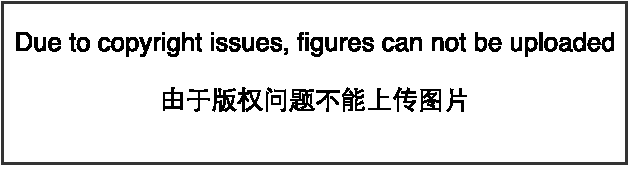
\includegraphics{figure.pdf}}
\else
\centerline{\includegraphics{Chapter7/figures/subnetworks}}
\fi
\caption{TODO}
\label{fig:chap7_subnetworks}
\end{figure}

% -- 251 --

回想一下使用\gls{bagging}学习,我们定义$k$个不同的模型,从训练集有替换采样构造$k$个不同的数据集,然后在训练集$i$上训练模型$i$。
\gls{dropout}的目标是在指数级数量的\gls{NN}上近似这个过程。
具体来说,训练中使用\gls{dropout},我们使用基于\gls{minibatch}的学习算法和小的步长,如\gls{GD}等。
我们每次在\gls{minibatch}加载一个样本,我们随机抽样应用与网络中所有输入和\gls{hidden_unit}的不同二值\gls{mask}。
对于每个单元,\gls{mask}是独立采样的。
\gls{mask}值为1的采样概率(导致包含一个单元)是训练开始前固定一个超参数。
它不是模型当前参数值或输入样本的函数。
通常一个输入单元包括的概率为$0.8$,一个\gls{hidden_unit}包括的概率为$0.5$。
然后,我们运行之前一样的前向传播、反向传播以及学习更新。
\figref{fig:chap7_dropout_fprop}说明了在\gls{dropout}下的前向传播。
\begin{figure}[!htb]
\ifOpenSource
\centerline{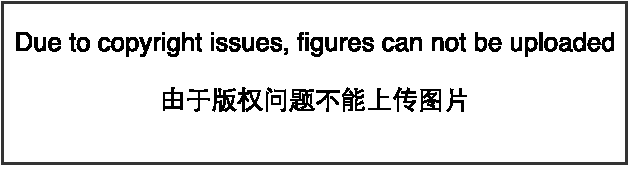
\includegraphics{figure.pdf}}
\else
\centerline{\includegraphics{Chapter7/figures/dropout_fprop}}
\fi
\caption{TODO}
\label{fig:chap7_dropout_fprop}
\end{figure}
% -- 252 --

更正式地说,假设一个\gls{mask}向量$\Vmu$指定被包括的单元,$J(\Vtheta, \Vmu)$是由参数$\Vtheta$和\gls{mask}$\Vmu$定义的模型代价。
那么\gls{dropout}训练在于最小化$\SetE_{\Vmu} J(\Vtheta, \Vmu)$。 
期望包含指数多的项,但我们可以通过抽样$\Vmu$获得梯度的无偏估计。

\gls{dropout}训练与\gls{bagging}训练不太一样。
在\gls{bagging}的情况下,所有模型是独立的。
在\gls{dropout}的情况下,模型是共享参数的,其中每个模型继承的父\gls{NN}参数的不同子集。
\gls{parameter_sharing}使得在有限可用的内存下代表指数数量的模型变得可能。
在\gls{bagging}的情况下,每一个模型被训练在其相应训练集上收敛。
在\gls{dropout}的情况下,通常大部分模型都没有显式地被训练,通常该模型很大,以致到宇宙毁灭都不能采样所有可能的子网络。
取而代之的是,可能的子网络的一小部分训练单个步骤,\gls{parameter_sharing}导致剩余的子网络能有好的参数设定。
这些是仅有的区别。
除了这些,\gls{dropout}与\gls{bagging}算法一样。
例如,每个子网络中遇到的训练集确实是有替换采样的原始训练集的一个子集。

\gls{bagging}\gls{ensemble}必须从所有成员的积累投票做一个预测。
在这种背景下,我们将这个过程称为\gls{inference}。
目前为止,\gls{bagging}和\gls{dropout}的描述中没有要求模型具有明确的概率。
现在,我们假定该模型的作用是输出一个概率分布。
在\gls{bagging}的情况下,每个模型$i$产生一个概率分布$p^{(i)}(y \mid \Vx)$。 
\gls{ensemble}的预测由这些分布的算术平均值给出,
\begin{align}
 \frac{1}{k} \sum_{i=1}^k p^{(i)}(y \mid \Vx).
\end{align}

在\gls{dropout}的情况下,通过\gls{mask}$\Vmu$定义每个子模型的概率分布$p(y \mid \Vx, \Vmu)$。
关于所有\gls{mask}的算术平均值由下式给出
\begin{align}
  \sum_{u} p(\Vmu) p(y \mid \Vx, \Vmu),
\end{align}
其中$p(\Vmu)$是训练时采$\Vmu$的概率分布。

% -- 254 --

因为这个求和包含指数多的项,除非在该模型的结构允许某种形式的简化,否则是不可能计算的。
目前为止,无法得知深度\gls{NN}是否允许任何可行的简化。
相反,我们可以通过采样近似\gls{inference},即平均许多\gls{mask}的输出。
即使是$10-20$个\gls{mask}就足以获得不错的表现。

然而,有一个更好的方法能得到一个不错的近似整个\gls{ensemble}的预测,且只需一个前向传播的代价。
要做到这一点,我们改用\gls{ensemble}成员的预测分布的几何平均而不是算术平均。
\cite{WardeFarley+al-ICLR2014}提出的论点和经验证据表明,在这个情况下几何平均与算术平均表现得差不多。

多个概率分布的几何平均不能保证是一个概率分布。
为了保证结果是一个概率分布,我们要求没有子模型给某一事件分配概率0,并重新标准化所得分布。
通过几何平均直接定义的非标准化概率分布由下式给出
\begin{align}
\tilde{p}_{\text{ensemble}}(y \mid \Vx) = \sqrt[2^d]{\prod_{\Vmu} p(y \mid \Vx, \Vmu)},
\end{align}
其中$d$是可被丢弃的单元数。
在这里,我们使用一个均匀分布的$\Vmu$以简化介绍,但非均匀分布也是可能的。
为了作出预测,我们必须重新标准化\gls{ensemble}:
\begin{align}
p_{\text{ensemble}}(y \mid \Vx)  = \frac{\tilde{p}_{\text{ensemble}}(y \mid \Vx)}
 {\sum_{y'}\tilde{p}_{\text{ensemble}}(y' \mid \Vx) }.
\end{align}
 
涉及\gls{dropout}的一个重要观点\citep{Hinton-et-al-arxiv2012}是,我们可以通过评估模型中$p(y \mid \Vx)$近似$ p_{\text{ensemble}}(y \mid \Vx) $:
该模型具有所有单元,但单元$i$输出的权重乘以包括单元$i$的概率。
这个修改的动机是捕获从该单元输出的正确期望值。
我们把这种方法称为\firstgls{weight_scaling_inference_rule}。
目前还没有在深度非线性网络上对这种近似推断规则的准确性作任何理论上的说法,但经验上表现得很好。

 % -- 255 --
 
因为我们通常使用一个$\frac{1}{2}$的包含概率,权重比例规则一般相当于在训练结束后将权重除$2$,然后像平常一样使用模型。
实现相同的结果的另一种方法是在训练期间将单元的状态乘$2$。
无论哪种方式,我们的目标是确保在测试时一个单元的期望总输入是与在训练时该单元的期望总输入是大致相同(即使近半单位在训练时丢失)。

对许多不具有非线性\gls{hidden_unit}的模型族,\gls{weight_scaling_inference_rule}是精确的。
举个简单的例子,考虑\gls{softmax}回归分类,其中由向量$\RVv$表示$n$个输入变量:
\begin{align}
 P(\RSy = \Sy \mid \RVv) = \text{softmax}\big(\MW^\top\RVv + \Vb\big)_y.
\end{align}
我们可以根据二值向量$\Vd$逐元素的乘法将一类子模型进行索引:
\begin{align}
P(\RSy = \Sy \mid \RVv; \Vd) = \text{softmax}\big(\MW^\top(\Vd \odot \RVv) + \Vb \big)_y.
\end{align}
\gls{ensemble}预测器被定义为重新标准化所有\gls{ensemble}成员预测的几何平均:
\begin{align} \label{eq:758pe}
P_{\text{ensemble}}(\RSy = \Sy \mid \RVv)  = \frac{\tilde{P}_{\text{ensemble}}(\RSy = \Sy \mid \RVv)}
 {\sum_{y'}\tilde{P}_{\text{ensemble}}(\RSy = \Sy' \mid \RVv) },
\end{align}
其中
\begin{align}
\tilde{P}_{\text{ensemble}}(\RSy=\Sy \mid \RVv) =
\sqrt[2^n]{\prod_{\Vd \in \{0,1\}^n} P(\RSy = \Sy \mid \RVv; \Vd)}.
\end{align}

为了证明\gls{weight_scaling_inference_rule}是精确的,我们简化$ \tilde{P}_{\text{ensemble}}$:
\begin{align}
\tilde{P}_{\text{ensemble}}(\RSy=\Sy \mid \RVv) =
\sqrt[2^n]{\prod_{\Vd \in \{0,1\}^n} P(\RSy = \Sy \mid \RVv; \Vd)} \\
= \sqrt[2^n]{\prod_{\Vd \in \{0,1\}^n} \text{softmax}(\MW^\top(\Vd \odot \RVv) + \Vb)_y} \\
= \sqrt[2^n]{\prod_{\Vd \in \{0,1\}^n} \frac{\exp (\MW_{y,:}^\top(\Vd \odot \RVv) + \Vb_y)}
{\sum_{y'}\exp (\MW_{y',;}^\top(\Vd \odot \RVv) + \Vb_{y'})}}\\
=  \frac{\sqrt[2^n]{\prod_{\Vd \in \{0,1\}^n}\exp (\MW_{y,:}^\top(\Vd \odot \RVv) + \Vb_y)}}
{ \sqrt[2^n] \prod_{\Vd \in \{0,1\}^n} \sum_{y'}\exp (\MW_{y',:}^\top(\Vd \odot \RVv) + \Vb_{y'})}
\end{align}

由于$\tilde P$将被标准化,我们可以放心地忽略那些相对$y$不变的乘法:
\begin{align}
\tilde{P}_{\text{ensemble}}(\RSy=\Sy \mid \RVv) &\propto 
\sqrt[2^n]{\prod_{\Vd \in \{0,1\}^n} \exp (\MW_{y,:}^\top(\Vd \odot \RVv) + \Vb_y)} \\
& = \exp \Bigg(\frac{1}{2^n} \sum_{\Vd \in \{0,1\}^n} \MW_{y,;}^\top(\Vd \odot \RVv) + \Vb_y \Bigg) \\
& = \exp \Big(\frac{1}{2}\MW_{y,:}^\top \RVv + \Vb_y \Big) .
\end{align}
将其代入\eqnref{eq:758pe},我们得到了一个权重为$\frac{1}{2}\MW$的\gls{softmax}分类器。

% -- 256 --

\gls{weight_scaling_inference_rule}在其他设定下也是精确的,包括条件正态输出的回归网络以及那些隐藏层不包含非线性的深度网络。
然而,\gls{weight_scaling_inference_rule}对具有非线性的深度模型仅仅是一个近似。
虽然这个近似尚未有理论上的分析,但在实践中往往效果很好。
\cite{Goodfellow-et-al-ICML2013}实验发现,\gls{ensemble}预测\gls{weight_scaling_inference_rule}可以比\gls{monte_carlo}近似工作得更好(在分类精度方面)。
即使允许\gls{monte_carlo}近似采样多达1000子网络时也比不过。
\cite{gal2015bayesian}发现一些模型可以通过二十个样本和\gls{monte_carlo}近似获得更好的分类精度。
似乎\gls{inference}近似的最佳选择是与问题相关的。

\cite{Srivastava14}显示,\gls{dropout}比其他标准的计算开销小的\gls{regularization} 项,如\gls{weight_decay}、过滤器范数约束和\gls{sparse}激活的\gls{regularization}更有效。
\gls{dropout}也可以与其他形式的\gls{regularization}合并,得到进一步的提升。

计算方便是\gls{dropout}的一个优点。
训练过程中使用\gls{dropout}产生$n$个随机二进制数与状态相乘,每个样本每次更新只需$\CalO(n)$的计算复杂度。
根据实现,也可能需要$\CalO(n)$的存储空间来持续保存这些二进制数(直到反向传播阶段)。
使用训练好的模型\gls{inference}时,计算每个样本的代价是与不使用\gls{dropout}一样的,尽管我们必须在开始运行\gls{inference}前将权重除以2。

% -- 257 --

\gls{dropout}的另一个显著优点是不怎么限制适用的模型或训练过程。
几乎在所有使用\gls{distributed_representation}且可以用\gls{SGD}训练的模型上都表现很好。
包括前馈神经网络、概率模型,如\gls{RBM}\citep{Srivastava14},以及\gls{RNN}\citep{Bayer-et-al-arXiv-2014,Pascanu-et-al-ICLR2014}。
许多其他差不多强大\gls{regularization}策略对模型结构的限制更严格。

虽然\gls{dropout}在特定模型上每一步的代价是微不足道的,但在一个完整的系统使用\gls{dropout}的代价可能非常显著。
因为\gls{dropout}是一个\gls{regularization}技术,它减少了模型的有效容量。
为了抵消这种影响,我们必须增大模型规模。
不出意外的话,使用\gls{dropout}时最佳验证集的误差会低很多,但这是以更大的模型和更多训练算法的迭代次数为代价换来的。
对于非常大的数据集,\gls{regularization}带来的泛化误差减少得很小。
在这些情况下,使用\gls{dropout}和更大模型的计算代价可能超过\gls{regularization}带来的好处。

只有极少的训练样本可用时,\gls{dropout}不会很有效。
在只有不到5000的样本的\ENNAME{Alternative Splicing}数据集上\citep{Xiong2011},贝叶斯神经网络\citep{Neal1996}比\gls{dropout}表现更好\citep{Srivastava14}。
当有其他未分类的数据可用时,无监督特征学习比\gls{dropout}更有优势。


\cite{Wager+al-2013}表明,当\gls{dropout}作用于\gls{linear_regression}时,相当于每个输入特征具有不同\gls{weight_decay}系数的$L^2$\gls{weight_decay}。 每个特征的\gls{weight_decay}系数的大小是由其方差来确定。
其他\gls{linear_model}有类似的结果。
而对于深度模型,\gls{dropout}与\gls{weight_decay}是不等同的。


使用\gls{dropout}训练时的随机性不是这个方法成功的必要条件。
它仅仅是近似所有子模型总和的一个方法。
\cite{WangManning-ICML2013-small}导出近似这种边缘分布的解析解。
他们的近似被称为\firstgls{fast_dropout}, 由于梯度计算中的随机性减小导致更快的收敛时间。
这种方法也可以在测试时应用,比\gls{weight_scaling_inference_rule}更合理地(但计算也更昂贵)近似所有子网络的平均。
\gls{fast_dropout}在小神经网络上的性能几乎与标准的\gls{dropout}相当,但在大问题上尚未产生显著地改善或尚未应用。

% -- 258 --

正如随机性对实现\gls{dropout}的\gls{regularization}效果不是必要的,这也不是充分的。
为了证明这一点,\cite{WardeFarley+al-ICLR2014}使用一种称为\firstgls{dropout_boosting}的方法设计了一个对照实验,与传统\gls{dropout}方法完全相同的噪声\gls{mask}, 但缺乏\gls{regularization}效果。
\gls{dropout_boosting}训练整个\gls{ensemble}以最大化训练集上的似然。
在相同意义上,传统的\gls{dropout}类似于\gls{bagging},这种方式类似于\gls{boosting}。
如预期一样,比较单一模型训练整个网络的情况,\gls{dropout_boosting}几乎没有\gls{regularization}效果。
这表明,\gls{dropout}\gls{bagging}的解释超过\gls{dropout}作为稳健性的噪音的解释。
当随机抽样的\gls{ensemble}成员相互独立地训练好后,\gls{bagging}\gls{ensemble}的\gls{regularization}效果才能达到。

\gls{dropout}启发其它以随机方法训练指数量级的共享权重的\gls{ensemble}。
\ENNAME{DropConnect}是\gls{dropout}的一个特殊情况,其中一个标量权重和单个\gls{hidden_unit}状态之间的每个乘积被认为是可以丢弃的一个单元\citep{Wan+al-ICML2013-small}。
随机\gls{pooling}是构造\gls{CNN}\gls{ensemble}的一种随机\gls{pooling}的形式(见\secref{sec:pooling}),其中每个卷积网络参与每个特征图的不同空间位置。
目前为止,\gls{dropout}仍然是最广泛使用的隐式\gls{ensemble}方法。

关于\gls{dropout}的一个重要见解是,通过随机行为训练网络并平均多个随机决定进行预测,通过\gls{parameter_sharing}实现了\gls{bagging}的一种形式。
早些时候,我们将\gls{dropout}描述为通过包括或排除单元形成模型\gls{ensemble}的\gls{bagging}。
然而,这种\gls{parameter_sharing}策略不一定要基于包括和排除。
原则上,任何一种随机的修改都是可接受的。
在实践中,我们必须选择能让\gls{NN}能够学习对抗的修改类型。
理想情况下,我们也应该使用可以快速近似\gls{inference}的模型类。
我们可以认为由向量$\Vmu$作为任何形式修改的参数,对于$\Vmu$所有可能的值训练$p(y \mid \Vx, \Vmu)$的\gls{ensemble}。
这里不要求$\Vmu$具有有限值。
例如,$\Vmu$可以是实值。
\cite{Srivastava14}表明,权重乘以$\Vmu \sim \CalN(1, \MI)$比基于二值\gls{mask} \gls{dropout}表现更好。
由于$\SetE[\Vmu] = 1$,标准网络自动实现\gls{ensemble}的近似\gls{inference},而不需要\gls{weight_scaling_inference_rule}。

% -- 259 --

到目前为止,我们已经介绍\gls{dropout}纯粹作为一种高效近似\gls{bagging}的手段。
然而,有比这更进一步的\gls{dropout}观点。
\gls{dropout}不仅仅是训练一个\gls{bagging}的\gls{ensemble}模型,
并且是共享\gls{hidden_unit}的\gls{ensemble}模型。
这意味着无论其它\gls{hidden_unit}是否在模型中,每个\gls{hidden_unit}必须都能够表现良好。
\gls{hidden_unit}必须准备好进行模型之间的交换和互换。
\cite{Hinton-et-al-arxiv2012-small}由生物学的想法受到启发:有性繁殖涉及到两个不同生物体之间交换基因,进化产生的压力使得基因不仅是良好的而且要准备好不同有机体之间的交换。
这样的基因和这些特点对环境的变化是非常稳健的,因为它们一定会正确适应任何一个有机体或模型不寻常的特性。
因此\gls{dropout}\gls{regularization}每个\gls{hidden_unit}不仅是一个很好的特征,更要在许多情况下良好的特征。
\cite{WardeFarley+al-ICLR2014}将\gls{dropout}与大\gls{ensemble}的训练相比并得出结论:相比独立模型的\gls{ensemble}获得的泛化误差,\gls{dropout}会提供的额外改进。

\gls{dropout}的强大大部分是由于被施加到\gls{hidden_unit}的\gls{mask}噪声,了解这一事实是重要的。
这可以看作是对输入内容的信息高度智能化的、自适应破坏的一种形式,而不是对输入原始值的破坏。
例如,如果模型学得通过鼻检测脸的\gls{hidden_unit}$h_i$,那么丢失$h_i$对应于擦除图像中有鼻子的信息。
模型必须学习另一种$h_i$,要么是鼻子存在的冗余编码,要么是脸部的另一特征,如嘴。
传统的噪声注入技术,在输入端加非结构化的噪声不能够随机地从脸部图像中抹去关于鼻子的信息,除非噪声的幅度大到几乎能抹去图像中所有的信息。
破坏提取的特征而不是原始值,让破坏过程充分利用该模型迄今获得的输入分布的所有知识。

\gls{dropout}的另一个重要方面是噪声是乘性的。
如果是固定规模的加性噪声,那么加了噪声$\epsilon$的修正线性\gls{hidden_unit}可以简单地学会使$h_i$变得很大(使增加的噪声$\epsilon$变得不显著)。
乘性噪声不允许这样病态地解决噪声鲁棒性问题。

% -- 260 --

另一种\gls{DL}算法,\gls{batch_normalization},在训练时向\gls{hidden_unit}引入加性和乘性噪声的方法重参数化模型。
\gls{batch_normalization}的主要目的是改善优化,但噪音具有\gls{regularization}的效果,有时使\gls{dropout}变得没有必要。
\gls{batch_normalization}将会在\secref{sec:batch_normalization}更详细的讨论。



\section{对抗训练}
\label{sec:adversarial_training}
在许多情况下,\gls{NN}在独立同分布的测试集上进行评估时已经达到人类表现。
因此,自然要怀疑这些模型在这些任务上是否获得了真正的人类层次的理解。
为了探测网络对底层任务的理解层次,我们可以搜索这个模型错误分类的例子。
\cite{Szegedy-ICLR2014}发现,精度达到人类水平的\gls{NN}在通过优化过程故意构造的点上的误差率接近\NUMTEXT{100\%},模型在这个输入点$\Vx'$的输出与附近的数据点$\Vx$非常不同。
在许多情况下,$\Vx'$与$\Vx$非常近似,人类观察者不知道原始样本和\firstgls{adversarial_example}之间的差异,但是网络会作出非常不同的预测。
见\figref{fig:chap7_panda_577}的例子。
\begin{figure}[!htb]
\ifOpenSource
\centerline{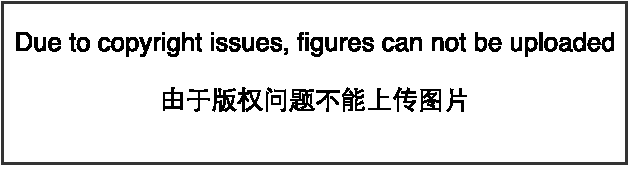
\includegraphics{figure.pdf}}
\else
\centerline{\includegraphics{Chapter7/figures/panda_577}}
\fi
\caption{TODO}
\label{fig:chap7_panda_577}
\end{figure}

% -- 261 --

\gls{adversarial_example}有很多的影响,例如计算机安全,这超出了本章的范围。
然而,它们在\gls{regularization}的背景下很有意思,因为我们可以通过\firstgls{adversarial_training}减少原有独立同分布的测试集上错误率——在对抗扰动的训练集样本上训练\citep{Szegedy-ICLR2014,Goodfellow-2015-adversarial}。


\cite{Goodfellow-2015-adversarial}表明,这些\gls{adversarial_example}的主要原因之一是过度线性。
\gls{NN}主要基于线性块构建的。
因此在一些实验中,他们实现的整体函数被证明是高度线性。
这些线性函数很容易优化。
不幸的是,如果一个线性函数具有许多输入,那么它的值可以非常迅速地改变。
如果我们用$\epsilon$改变每个输入,那么权重为$\Vw$线性函数可以改变$\epsilon \norm{\Vw}_1$之多,如果$\Vw$是高维的这会是一个非常大的数。
\gls{adversarial_training}通过鼓励网络在训练数据附近的局部区域恒定来限制这一高度敏感的局部线性行为。
这可以被看作是明确地向监督\gls{NN}引入局部恒定的先验的方法。

对抗训练有助于说明积极\gls{regularization}与大型函数族结合的力量。
纯粹的\gls{linear_model},如\gls{logistic_regression},由于他们被限制为线性而无法抵抗\gls{adversarial_example}。
\gls{NN}是能够将函数从接近线性转化为局部近似恒定,从而可以灵活地捕获到训练数据中的线性趋势同时学习抵抗局部扰动。

\gls{adversarial_example}也提供了实现半监督学习的一种手段。
与数据集中的标签不相关联的点$\Vx$处,模型本身为其分配一些标签$\hat y$。
模型的标记$\hat y$未必是真正的标签,但如果模型是高品质,那么$\hat y$提供真正标签的可能性很大。
我们可以搜索一个\gls{adversarial_example}$\Vx'$,导致分类器输出一个标签$y'$且$y' \neq \hat y$。
不使用真正的标签,而是由训练好的模型提供标签产生的\gls{adversarial_example}称为\firstgls{virtual_adversarial_example}\citep{miyato2015distributional}。
分类器可以被训练成对$\Vx$和$\Vx'$分配相同的标签。
这鼓励分类器学习一个沿着未标签数据所在流形上任意微小变化都是鲁棒的函数。
驱动这种方法的假设是,不同的类通常位于分离的流形上,并且小的扰动不能从一类的流形跳到另一个类的流形。

% -- 262 -- 

%%%%%%%%%%%%%%%%%%%%%%%%%%%%%%%%%%%%%%%%%%%%%%
%       Hard to translate
%%%%%%%%%%%%%%%%%%%%%%%%%%%%%%%%%%%%%%%%%%%%%%
\section{\glsentrytext{tangent_distance}、\glsentrytext{tangent_prop}和流形切分类}
\label{sec:tangent_distance_tangent_prop_and_manifold_tangent_classifier}
许多\gls{ML}的目标旨在假设数据位于低维流形附近来克服维数灾难,如\secref{sec:manifold_learning}描述。

一个利用流形假设的早期尝试是\firstgls{tangent_distance}算法\citep{Simard93-small,Simard98}。
它是一种非参数最近邻算法,其中度量使用的不是通用的欧几里德距离,而是是从邻近流形关于聚集概率的知识导出的。
这假设我们正在尝试的分类样本,且同一流形上的样本共享相同的类别。
由于分类器应该对变化的局部因素(对应于流形上的移动)不变,将点$\Vx_1$和$\Vx_2$分别所在的流形$M_1$和$M_2$的距离作为点$\Vx_1$和$\Vx_2$的最近邻距离是合理的。
尽管这可能是在计算上是困难(它需要解决一个找到$M_1$和$M_2$最近对点的优化问题),一种廉价的替代是局部合理的,即使用$\Vx_i$点处切平面近似$M_i$,并测量两条切平面或一个切平面和点的距离。
可以通过求解一个低维线性系统(流形的维数)实现。
当然,这种算法需要制定一个的切向量。

受相关启发,\firstgls{tangent_prop}算法\citep{Simard92-short}(\figref{fig:chap7_mtc_color})训练带有额外惩罚的\gls{NN}分类器,使\gls{NN}的每个输出$f(\Vx)$对已知的变化因素是局部不变的。
这些变化因素对应于沿着的相同样本聚集的流形的移动。
局部不变性是通过要求$\nabla_{\Vx} f(\Vx)$与已知流形的切向$\Vv^{(i)}$正交实现的,或者等价地通过\gls{regularization}惩罚$\Omega$使$f$在$\Vx$的$\Vv^{(i)}$方向的导数是小的:
\begin{align} \label{eq:767}
 \Omega(f) = \sum_i \Big((\nabla_{\Vx} f(\Vx)^\top \Vv^{(i)}) \Big)^2 .
\end{align}
这个\gls{regularization}项当然可以通过适当的超参数缩放,并且对于大多数\gls{NN},我们将需要对许多输出求和(此处为描述简单,$f(\Vx)$为唯一输出)。
与\gls{tangent_distance}算法一样,切向量推导先验,通常是从变换,如平移、旋转和缩放图像的效果获得形式知识。
\gls{tangent_prop}不仅用于监督学习\citep{Simard92-short},还在强化学习\citep{Thrun-NIPS1994}中有所应用。
\begin{figure}[!htb]
\ifOpenSource
\centerline{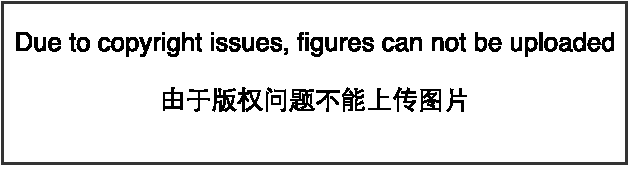
\includegraphics{figure.pdf}}
\else
\centerline{\includegraphics{Chapter7/figures/mtc_color}}
\fi
\caption{TODO}
\label{fig:chap7_mtc_color}
\end{figure}
% -- 263 --

\gls{tangent_prop}与数据集增强密切相关。
在这两种情况下,该算法的用户通过指定一组不改变网络输出的转换,编码其先验知识。
不同的是在数据集增强的情况下,网络是显式地训练正确分类这些施加大量变换后产生的不同输入。
\gls{tangent_prop}不需要显式访问一个新的输入点。
取而代之,它解析地对模型\gls{regularization}在对应于指定转换的方向抵抗扰动。
虽然这种分析方法是聪明优雅的,它有两个主要的缺点。
首先,模型的\gls{regularization}只能抵抗无穷小扰动。
显式的数据集增强能对抗较大扰动。
二是无限小的做法对基于\gls{ReLU}的模型是困难的。
这些模型只能通过关闭单元或缩小它们的权重才能缩小它们的导数。
他们不能像\ENNAME{sigmoid}或\ENNAME{tanh}单元一样通过大的权重在高值处饱和以收缩导数。
数据集增强在\gls{ReLU}上工作得很好,因为修正单元的不同子集针对每一个原始输入不同的转换版本激活。

% -- 264 --

\gls{tangent_prop}也涉及到\gls{double_backprop}\citep{DruckerLeCun92}和\gls{adversarial_training}\citep{Szegedy-et-al-arxiv2014,Goodfellow-2015-adversarial}。
\gls{double_backprop}\gls{regularization}\gls{jacobian}要小,而\gls{adversarial_training}找到原输入附近的点,训练模型以在这些点产生与原来输入相同的输出。
\gls{tangent_prop}和手工指定转换的数据集增强都要求模型对输入变化的某些特定的方向是不变的。
\gls{double_backprop}和\gls{adversarial_training}都要求模型对输入所有方向中的变化(只要该变化较小)都应当是不变的。
正如数据集增强是\gls{tangent_prop}非无限小的版本,\gls{adversarial_training}是\gls{double_backprop}非无限小的版本。

流形切面分类器\citep{Dauphin-et-al-NIPS2011}无需知道切线向量的先验。
正如我们将在\chapref{chap:autoencoders}看到,\gls{AE}可以估算流形的切向量。
流形切面分类器使用这种技术来避免用户指定切向量。
如\figref{fig:chap14_cifar_cae}所示,这些估计的切向量超出了图像(如转化、旋转和缩放)几何的经典不变,还必须掌握因为特定对象(如移动身体的部分)的因素。
因此根据流形切面分类提出的算法是简单:
(1)使用\gls{AE}通过无监督学习来学习流形的结构,以及(2)如\gls{tangent_prop}(\eqnref{eq:767})一样使用这些切面\gls{regularization}\gls{NN}分类器。

在本章中,我们已经描述了大多数用于\gls{regularization}\gls{NN}的通用策略。
\gls{regularization}是\gls{ML}的中心主题,因此将定期在其余各章中重新回顾。
\gls{ML}的另一个中心主题是优化,将在下章描述。

% -- 265 --
